\documentclass[12pt]{article}\usepackage[]{graphicx}\usepackage[dvipsnames]{xcolor}
% maxwidth is the original width if it is less than linewidth
% otherwise use linewidth (to make sure the graphics do not exceed the margin)
\makeatletter
\def\maxwidth{ %
  \ifdim\Gin@nat@width>\linewidth
    \linewidth
  \else
    \Gin@nat@width
  \fi
}
\makeatother

\definecolor{fgcolor}{rgb}{0.345, 0.345, 0.345}
\newcommand{\hlnum}[1]{\textcolor[rgb]{0.686,0.059,0.569}{#1}}%
\newcommand{\hlstr}[1]{\textcolor[rgb]{0.192,0.494,0.8}{#1}}%
\newcommand{\hlcom}[1]{\textcolor[rgb]{0.678,0.584,0.686}{\textit{#1}}}%
\newcommand{\hlopt}[1]{\textcolor[rgb]{0,0,0}{#1}}%
\newcommand{\hlstd}[1]{\textcolor[rgb]{0.345,0.345,0.345}{#1}}%
\newcommand{\hlkwa}[1]{\textcolor[rgb]{0.161,0.373,0.58}{\textbf{#1}}}%
\newcommand{\hlkwb}[1]{\textcolor[rgb]{0.69,0.353,0.396}{#1}}%
\newcommand{\hlkwc}[1]{\textcolor[rgb]{0.333,0.667,0.333}{#1}}%
\newcommand{\hlkwd}[1]{\textcolor[rgb]{0.737,0.353,0.396}{\textbf{#1}}}%
\let\hlipl\hlkwb

\usepackage{framed}
\makeatletter
\newenvironment{kframe}{%
 \def\at@end@of@kframe{}%
 \ifinner\ifhmode%
  \def\at@end@of@kframe{\end{minipage}}%
  \begin{minipage}{\columnwidth}%
 \fi\fi%
 \def\FrameCommand##1{\hskip\@totalleftmargin \hskip-\fboxsep
 \colorbox{shadecolor}{##1}\hskip-\fboxsep
     % There is no \\@totalrightmargin, so:
     \hskip-\linewidth \hskip-\@totalleftmargin \hskip\columnwidth}%
 \MakeFramed {\advance\hsize-\width
   \@totalleftmargin\z@ \linewidth\hsize
   \@setminipage}}%
 {\par\unskip\endMakeFramed%
 \at@end@of@kframe}
\makeatother

\definecolor{shadecolor}{rgb}{.97, .97, .97}
\definecolor{messagecolor}{rgb}{0, 0, 0}
\definecolor{warningcolor}{rgb}{1, 0, 1}
\definecolor{errorcolor}{rgb}{1, 0, 0}
\newenvironment{knitrout}{}{} % an empty environment to be redefined in TeX

\usepackage{alltt}
\usepackage{amsmath,amsfonts,amssymb,graphicx,authblk}
\usepackage[font={footnotesize,singlespacing},labelfont=bf]{caption}
\usepackage{titlesec,blkarray, bm} 
\usepackage{float,afterpage}
\usepackage[running,mathlines]{lineno}
\usepackage[vmargin=1in,hmargin=1in]{geometry}
\usepackage[authoryear,sort]{natbib}
\usepackage[dvipsnames]{xcolor}
\usepackage[nodisplayskipstretch]{setspace} 
\usepackage{hyperref}
\usepackage[section]{placeins}
\usepackage{gensymb}
\usepackage{enumitem}
\usepackage{orcidlink}
\setlist{topsep=.125em,itemsep=-0.15em,leftmargin=0.75cm}
\setlength{\parindent}{0.35in}

\usepackage[sc]{mathpazo} %Like Palatino with extensive math support
\usepackage[subtle]{savetrees}

\usepackage{lineno}
%\renewcommand{\refname}{Literature Cited}
%\renewcommand{\floatpagefraction}{0.9}
%\renewcommand{\topfraction}{0.99}
%\renewcommand{\textfraction}{0.05}

\clubpenalty = 10000
\widowpenalty = 10000

\sloppy 

\usepackage{ifpdf}
\ifpdf
\DeclareGraphicsExtensions{.pdf,.png,.jpg}
\usepackage{epstopdf}
\else
\DeclareGraphicsExtensions{.eps}
\fi

\graphicspath{{/Users/jm200/Library/CloudStorage/Dropbox/Miller Lab/github/POAR-Forecasting/Manuscript/Figures/}}
\newcommand{\tom}[2]{{\color{red}{#1}}\footnote{\textit{\color{red}{#2}}}}
\newcommand{\jacob}[2]{{\color{blue}{#1}}\footnote{\textit{\color{blue}{#2}}}}
%\doublespacing



% I cannot get \orcidlink working on my computer so for now replacing this with \textit

%-------------------------------------------------------------------------
\title{Forecasting range shifts of a dioecious plant species under climate change}
\author[1]{Jacob K. Moutouama\,\textit{0000-0003-1599-1671} \thanks{Corresponding author: jmoutouama@gmail.com}}
\author[2]{Aldo Compagnoni\,\textit{0000-0001-8302-7492}}
\author[1]{Tom E.X. Miller\,\textit{0000-0003-3208-6067}}
\affil[1]{Program in Ecology and Evolutionary Biology, Department of BioSciences, Rice University, Houston, TX USA}
\affil[2]{Institute of Biology, Martin Luther University Halle-Wittenberg, Halle, Germany; and German Centre for Integrative Biodiversity Research (iDiv), Leipzig, Germany}
\date{} % clear date
%\renewcommand\Authands{ and }

\sloppy

%-------------------------------------------------------------------------
\IfFileExists{upquote.sty}{\usepackage{upquote}}{}
\begin{document}
%\SweaveOpts{concordance=TRUE}
\renewcommand{\baselinestretch}{1.2}
\maketitle
% \bigskip 
%45 character limit on running head
\noindent\textbf{Running header:} Forecasting range shifts
\bigskip 

\noindent\textbf{Keywords:} demography, forecasting, global warming, matrix projection model, population dynamics, sex ratio, range limits

\bigskip 
\noindent\textbf{Submitted to:} \textit{Ecology letters} (Letter)

\bigskip 
\noindent\textbf{Data accessibility statement:} All data used in this paper are  publicly available and cited appropriately \citep{dryaddata}. 
Should the paper be accepted, all computer scripts supporting the results will be archived in a Zenodo package, with the DOI included at the end of the article. 
During peer review, our code (Stan, Bash and R) is available at \url{https://github.com/jmoutouama/POAR-Forecasting}. 

\bigskip 
\noindent\textbf{Conflict of interest statement:} None.

\bigskip
\noindent\textbf{Authorship statement:}
J.K.M., A.C. and T.E.X.M. designed the study.
A.C. and T.E.X.M. collected the data. 
All authors conducted the statistical analyses and modeling.
J.K.M. drafted the manuscript, and T.E.X.M contributed to revisions.

\bigskip
\noindent\textbf{Abstract:}\\
\noindent\textbf{Main Text:}\\
\noindent\textbf{Figures: 6}\\
\noindent\textbf{Tables: 0}\\
\noindent\textbf{References: 106}

\newpage
%\SweaveOpts{concordance=TRUE}
\linenumbers
%-------------------------------------------------------------------------
\spacing{1.25}
\section*{Abstract}
%150 words limit for Ecology letter. The number now is 155
%Tom made changes here that increase word count
Global climate change has triggered an urgent need for predicting the reorganization of Earth's biodiversity.
Currently, the vast majority of models used to forecast population viability and range shifts in response to climate change ignore the complication of sex structure, and thus the potential for females and males to differ in their sensitity to climate drivers. 
% For dioecious species, it is unclear how commonly unique climate sensitivities of females and males could influence projections for species-level responses to climate change. 
We developed demographic models of range limitation, parameterized from geographically distributed common garden experiments, with females and males of a dioecious grass species (\textit{Poa arachnifera}) throughout and beyond its range in the south-central U.S. 
Female-dominant and two-sex model versions both predict that future climate change will alter population viability and will induce a poleward niche shift beyond current northern limits.
However, the magnitude of niche shift was underestimated by the female-dominant model, because females have broader temperature tolerance than males and become mate-limited under female-biased sex ratios.
Our result illustrate how explicit accounting for both sexes could enhance population viability forecasts and conservation planning for dioecious species in response to climate change.

%--------------------------------------------------------------------
\newpage
\section*{Introduction}
Rising temperatures and extreme drought events associated with global climate change are leading to increased concern about how species will become redistributed across the globe under future climate conditions \citep{bertrand2011changes,gamelon2017interactions,smith2024extreme}.
Species' range limits, when not driven by dispersal limitation, should generally reflect the limits of the ecological niche \citep{lee2016synthesis}.
Niches and geographic ranges are often limited by climatic factors including temperature and precipitation \citep{sexton2009evolution}. 
Therefore, any substantial changes in the magnitude of these climatic factors could impact population viability, with implications for range expansions or contractions based on which regions of a species' range become more or less suitable  \citep{davis2001range, pease1989model}. 

%Dioecious species (most animals and ca. 7\% of plant species) might be particularly vulnerable to the influence of climate change because they often display skewed sex ratios that are generated or reinforced by sexual niche differentiation, i.e., the distinct responses of females and males to shared climate drivers) \citep{Tognetti2012}. 
Forecasting range shifts for dioecious species (most animals and ca. 7\% of plant species) is complicated by the potential for each sex to respond differently to climate variation \citep{Tognetti2012,pottier2021sexual,hultine2016climate,morrison2016causes}. 
\tom{}{Something this paragraph is missing is a mechanistic explanation for why females and males may have different climate sensitivity, likely something about costs of reproduction. This would be a good place for a sentence or two that addresses this.}
Accounting for sexual niche differentiation is a long-standing challenge in accurately predicting which sex will successfully track environmental change and how this will impact population viability and range shifts \citep{jones1999sex,gissi2023exploring}. 
Populations in which males are rare under current climatic conditions could experience low reproductive success due to sperm or pollen limitation that may lead to population decline in response to climate change that disproportionately favors females \citep{eberhart2017sex}.
In contrast, climate change could expand male habitat suitability (e.g. upslope movement), which might increases seed set for pollen-limited females and favor range expansion \citep{petry2016sex}. 
\tom{Across dioecious plants, studies suggest that future climate change toward hotter and drier conditions may favor male-biased sex ratios \citep{field2013comparative,hultine2016climate}. }{I am not sure if this is the best spot for it, but I think this prediction from the literature is relevant to bring up in the Intro.}
Although the response of species to climate warming is an urgent and active area of research, few studies have disentangled the interaction between sex and climate drivers to understand their combined effects on population dynamics and range shifts, despite calls for such an approach \citep{hultine2016climate,gissi2023exploring}.

The vast majority of theory and models in population biology, including those used to forecast biodiversity responses to climate change, ignore the complication of sex structure \citep[but see][] {pottier2021sexual,ellis2017does,Elena}.
Traditional approaches instead focus exclusively on females, assuming that males are in sufficient supply as to never limit female fertility. 
In contrast, ``two-sex'' models are required to fully account for demographic differences between females and males and sex-specific responses to shared climate drivers \citep{gerber2014two,miller2011sex}. 
Sex differences in maturation, reproduction, and mortality schedules can generate skew in the operational sex ratio (OSR; sex ratio of individuals available for mating) even if the birth sex ratio is 1:1 \citep{eberhart2017sex,shelton2010ecological}. 
Climate and other environmental drivers can therefore influence the OSR via their influence on sex-specific demographic rates. 
In a two-sex framework, demographic rates both influence and respond to the OSR in a feedback loop that makes two-sex models inherently nonlinear and more data-hungry than corresponding female-dominant models. 
Given the additional complexity and data needs, forecasts of range dynamics for dioecious species under future climate change that explicitly account for females, males, and their inter-dependence are limited \citep{petry2016sex,lynch2014climate}.


% \tom{Climate change can influence dioecious populations via shifts in sex ratio.}{This paragraph is really good but notice that the topic sentence (and much that follows) is largely redundant with the first paragraph. I would suggest creating clearer distinction between paragraphs.} 
% Females and males may respond differently to climate change, especially in species where there is sexual niche differentiation \citep{gissi2023exploring,gissi2023sex,hultine2016climate}. 
% This sex-specific response to climate change may help one sex to succeed in extreme climatic conditions rather than the other sex \citep{zhao2012sex, burli2022environmental} leading to a skewness in the operational sex ratio (relative number of males and females as available mates) \citep{eberhart2017sex}.
% For example, experiments in two populations of Atlantic marine copepods (\textit{Acartia tonsa}) revealed that male survival was more sensitive to increasing temperatures than female survival \citep{sasaki2019complex}.
% In other species, such as \textit{Pteropus poliocephalus} or \textit {Populus cathayana}, females showed lower survival than males in response to high temperature \citep{welbergen2008climate,zhao2012sex}. 
% Sex-specific responses to climate drivers have the potential to influence population viability under global change because skew in the operational sex ratio can limit reproduction through mate scarcity \citep{petry2016sex}.

Tracking the impact of climate change on  population viability ($\lambda$) and distributional limits of dioecious taxa depends on our ability to build mechanistic models that take into account the spatial and temporal context of sex specific response to climate change, while accounting for sources of uncertainty \citep{davis2001range,evans2016towards,czachura2020demographic}.
Structured population models built from demographic data collected from geographically distributed observations or common garden experiments provide several advantages for studying the impact of climate change on species' range shifts \citep{merow2017climate,schwinning2022common,schultz2022climate}.
First, demographic models link individual-level life history events (mortality, development, and regeneration) to population demography, allowing the investigation of factors explaining vital rate responses to environmental drivers \citep{ehrlen2015predicting,louthan2022climate,dahlgren2016demography}. 
Second, demographic models have a natural interface with %experimental treatments that can isolate spatial and temporal correlations between environmental factors, thus overcoming a main disadvantage with many types of correlative studies \citep{leicht2007comparative}. 
%Third, demographic models are typically constructed from 
statistical estimation individual-level vital rates that provide quantitative measures of uncertainty and isolate different sources of variation, features that can be propagated to population-level predictions \citep{elderd2016quantifying}.\tom{}{I cut the sentence about experiments because I don't think our data really exemplify this. While we did do an experiment, we did not manipulate climate, so we are subject to the same correlations as observational studies.}
% The uncertainty around lambda can be used to estimate the probability of self-sustaining populations, conditional on different factors of the environment.
Finally, structured demographic models can be used to identify which aspects of climate are the most important drivers of population dynamics.
For example, Life Table Response Experiments (LTRE) built from structured models have become widely used to understand the relative importance of covariates in explaining variation in population growth rate  \citep{ellner2016data,hernandez2023exact}.\tom{}{I think LTRE is a relatively small part of the paper so I suggested reducing the amount of text on it here.}
%LTRE is also used to get a mechanistic understanding of how a given treatment (eg. temperature or precipitation) could affect population dynamics through unique vital rate responses \citep {caswell1989analysis,o2024nonlinear,morrison2007demographic,iler2019reproductive}. %\jacob{}{Yes I don't want to get distracted by SDMs. The story is still interesting without bashing the SDMs studies. That being said, I showed the advantage of using demographic models over traditional correlative approaches. Line 59-62)}
% At their range edge where climatic conditions are expected to be less favorable, if dioecious species populations are non-viable in response to climate change, global warming will induce range contraction in dioecious species.
% In reverse, if populations at the edge are viable habitats in response to global warming, dioecious species populations could shift their range and relocate to more favorable and thereby favored range expansion. 

In this study, we combine geographically-distributed common garden experiments, hierarchical Bayesian statistical modeling, two-sex population projection modeling, and climate back-casting and forecasting to understand demographic responses to climate change and their implications for past, present, and future range dynamics. 
Our work focused on the dioecious plant Texas bluegrass (\textit{Poa arachnifera}), which is distributed along environmental gradients in the south-central U.S. corresponding to variation in temperature across latitude and precipitation across longitude (Fig. \ref{fig:study_design}). 
This region has experienced rapid climate warming since 1900 and this is projected to continue through the end of the century (Fig. \ref{Sup:temp_variation}).  
Our previous study showed that, despite evidence for differentiation of climatic niche between sexes, the female niche mattered the most in driving longitudinal range limits of Texas bluegrass \citep{miller2022two}. 
However, that study used a single proxy variable (longitude) to represent environmental variation related to aridity and did not consider variation in temperature, which is the much stronger dimension of forecasted climate change in this region (Fig. \ref{Sup:temp_variation},\ref{Sup:pr_variation}). 
Developing a rigorous forecast for the implications of future climate change requires that we transition from climate-implicit to climate-explicit treatment of multiple environmental drivers as we do here.
Leveraging the power of Bayesian inference, we take a probabilistic view of past, present, and future range limits by quantifying the probability of population viability ($Pr(\lambda\ge1)$) in relation to climate drivers of demography, given uncertainty arising from multiple sources of estimation and process error. %using Markov Chain Monte Carlo (MCMC) can be utilized to infer species niche which is defined as the range of resources and conditions allowing its populations of self-sustaining populations, conditional on different factors of the environment \citep{maguire1973niche,hutchinson1978introduction,diez2014probabilistic}
Specifically, we asked: 
\begin{enumerate}
	\item What are the sex-specific vital rate responses to variation in temperature and precipitation across the species' range?
	\item How do sex-specific vital rates combine to determine the influence of climate variation on population growth rate ($\lambda$)?
	\item What is the impact of climate change on operational sex ratio throughout the range?
	\item What are the historical and projected dynamics of the Texas bluegrass geographic niche and how does accounting for sex structure modify these predictions?
\end{enumerate}

%--------------------------------------------------------------------
\section*{Materials and methods}
\subsection*{Study species}
Texas bluegrass (\textit{Poa arachnifera}) is a dioecious perennial, summer-dormant cool-season (C3) grass that occurs in the south-central U.S. (Texas, Oklahoma, and southern Kansas) (Figure \ref{fig:study_design}) \citep{hitchcock1971manual}\jacob{}{I have updated the map}. 
Latitudinal limits of the Texas bluegrass distribution span 7.74 \degree C to 16.94 \degree C of temperature during the dormant season and 24.38 \degree C to 28.80 \degree C  during the dormant season. 
Longitudinal limits span 244.9 mm to 901.5 mm of precipitation during the growing season and 156.3 mm to 373.3 mm. 
Texas bluegrass grows between October and May (growing season), with onset of dormancy often from June to September (dormant season) \citep{kindiger2004interspecific}. 

Biological sex in Texas blueegrass is genetically based and the birth (seed) sex ratio is 1:1 \citep{renganayaki2005identification}. 
Females and males are morphologically indistinguishable except for their inflorescences. 
Flowering occurs in May and the species is wind pollinated \citep{hitchcock1971manual}. 
Surveys of 22 natural populations throughout the species' distribution indicated that operational sex ratio (the female fraction of flowering plants) ranged from 0.007 to 0.986 with a mean of 0.404 \citep{miller2022two}. 

\subsection*{Common garden experiment}
We set up a common garden experiment throughout and beyond the range of Texas bluegrass to quantify sex-specific demographic responses to climate. 
Details of the experimental design are provided in \cite{miller2022two}; we provide a brief overview here. 
The experiment was installed at 14 sites throughout and, in some cases, beyond the species' natural range (Figure \ref{fig:study_design}).
At each site, we established 14 blocks. 
For each block we planted the same number of plant from each sex (three female and three male individuals) that were clonally propagated from females and males from eight natural source populations (Figure \ref{fig:study_design}); because sex is genetically-based, clones never deviated from their expected sex. 
The experiment was established in November 2013 and was censused in May of 2014, 2015, and 2016. 
At each census, we collected individual demographic data including survival (alive or dead), size (number of tillers), and number of panicles (reproductive inflorescences). 
For the analyses that follow, we focus on the 2014-15 and 2015-16 transitions years, since the start of the experiment did not include the full 2013-14 transition year.

\begin{figure}[H]
  \begin{center}
    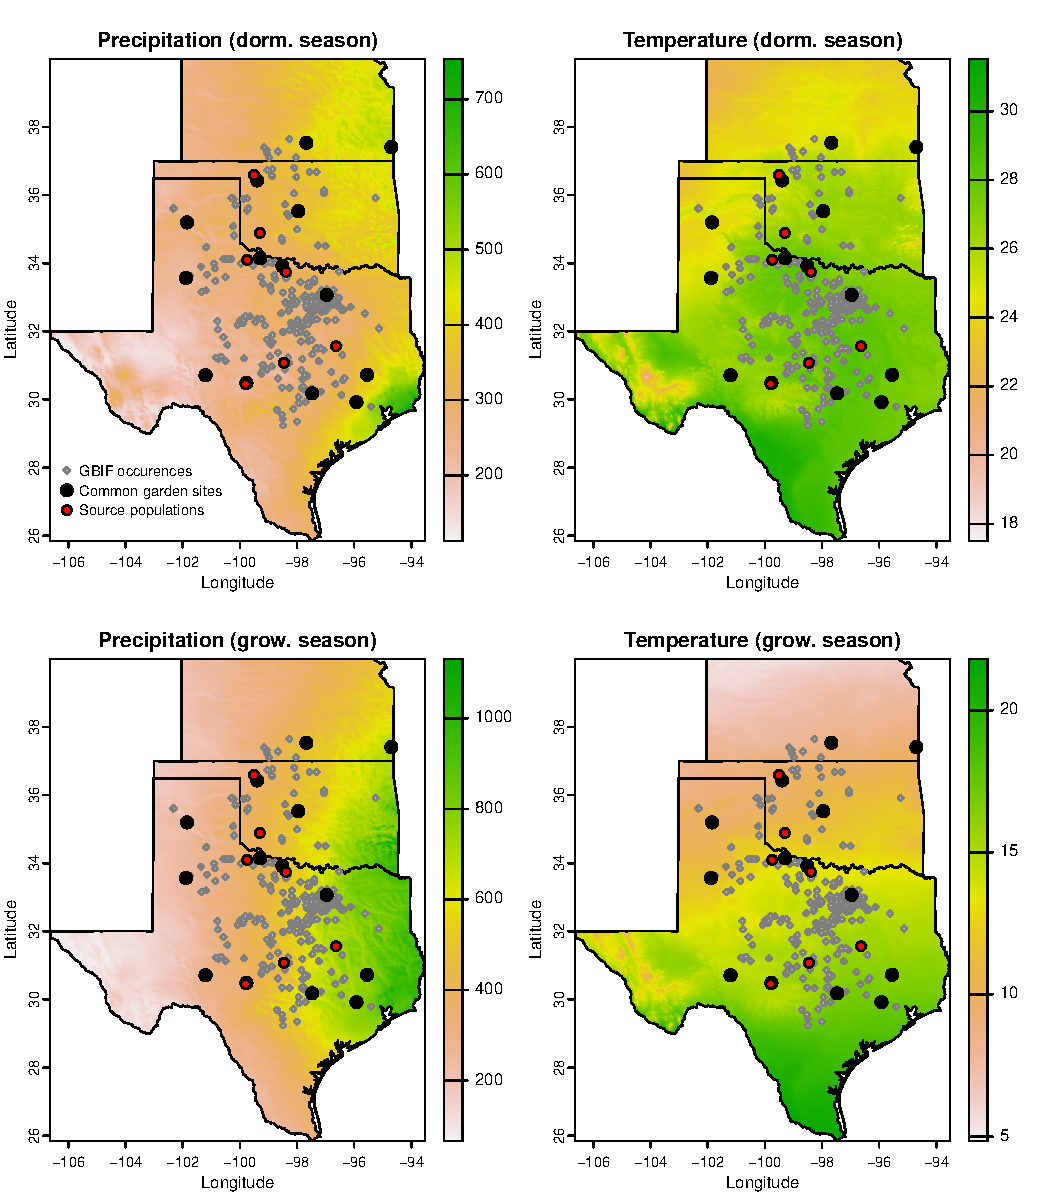
\includegraphics[width=0.90\linewidth]{Figures/POAR_survey_garden_map.pdf}
  \caption{\textbf{Maps of 30-year (1990-2019) normal climate and study sites used for demographic monitoring of \emph{Poa arachnifera} in Texas, Kansas and Oklahoma in the United States}.
  Precipitation of growing and precipitation of dormant season are in mm, temperature of the dormant and temperature of growing season are in \degree C.
  We surveyed 22 natural populations (grey diamond).
  The common garden sites were installed on 14 sites (black circle) collected from 7 sources populations (red circle).
  See also (Figure \ref{Sup:temp_variation}, Figure \ref{Sup:pr_variation}) for more details about climate variation across the study sites since the beginning of last century.}
  \label{fig:study_design}
  \end{center}
\end{figure}

\subsection*{Climatic data collection}
We gathered downscaled monthly temperature and precipitation for each site from Chelsa to describe observed climate conditions during our study period \citep{karger2017climatologies}.
These climate data were used as covariates in vital rate regressions. 
%We prefer temperature and precipitation because they capture the most the climate in the study region \colorbox{BurntOrange}{Source}. 
We aligned the climatic years to match demographic transition years (June 1 -- May 31) rather than calendar years.
Based on the natural history of this summer-dormant cool-season species, we divided each transition year into dormant (June 1 through September 30) and growing (October 1 through May 31) seasons. 
% The 2014-15 transition year was substantially wetter and cooler across the study region than 2015-16, especially during the growing season (Fig.\ref{Sup:climate_variation}), so our study design provides both spatial and inter-annual coverage of climate variables. 

To back-cast and forecast demographic responses to changes in climate throughout the study region, we downloaded projection data for three 30-year periods: ``past'' (1901-1930), ``current'' (1990-2019) and ``future'' (2070-2100).
Data for future climatic periods were downloaded from four general circulation models (GCMs) selected from the Coupled Model Intercomparison Project Phase 5 (CMIP5). 
The GCMs are: Model for Interdisciplinary Research on Climate (MIROC5), Australian Community Climate and Earth System Simulator (ACCESS1-3), Community Earth System Model (CESM1-BGC), Centro Euro-Mediterraneo sui Cambiamenti Climatici Climate Model (CMCC-CM).
All the GCMs were also downloaded from chelsa \citep{sanderson2015representative}.
We evaluated future climate projections from two scenarios of representative concentration pathways (RCPs): RCP4.5, an intermediate-to-pessimistic scenario assuming a radiative forcing amounting to 4.5 $W m^{-2}$ by 2100, and RCP8.5, a pessimistic emission scenario which projects a radiative forcing of 8.5 $W m^{-2}$ by 2100 \citep{thomson2011rcp4, schwalm2020rcp8}. 

Projection data for the three 30-year periods had warmer or colder conditions than observed in our experiment (Figure \ref{Sup:projectionMIROC}, Figure \ref{Sup:projectionACCESS}, Figure \ref{Sup:projectionCESM1}, Figure \ref{Sup:projectionCMCC}). 
However, the observed period was substantially wetter and cooler across the study region than 2015-16, especially during the growing season (Figure \ref{Sup:climate_variation}), so our study design provides both spatial and inter-annual coverage of climate variables. 


\subsection*{Sex specific demographic responses to climate}
\jacob{}{ I have reduced the redundancy between the two paragraphs and added the biological rationale for the model.  I hope that the explaination I added provided a clarification about why I did not use model selection.}
We used individual level measurements of survival, growth (number of tillers), flowering, number of panicles to develop Bayesian linear mixed effect models describing how each vital rate varies as a function of sex, size, and four climate covariates (precipitation and temperature of growing and dormant season). 
We kept the four climate covariates in the mixed effect models because each climatic variable describes different aspect of climate that could be important for the species persistence across its range. 
Vital rate models were fit with second-degree polynomial functions and with the same linear predictors for the expected value ($\mu$)(Eq.\ref{eq:mu}).
The second-degree polynomial was included because we expected that climate would affect vital rates through a hump-shaped relationship assuming that (i) the center of the range is the optimum range for the species (ii) and climate sets limits on whether habitats will be suitable for the study species.
We also included the interaction effect of temperature and precipitation for each season to understand the synergistic effect of both variables on population demography. 
We centered and standardized all climatic predictors to facilitate model convergence.
Size (number of tillers) was on a natural logarithm scale. 
\begin{align}\label{eq:mu}
\begin{split}
\mu = \beta_{0} + \beta_{1}size + \beta_{2}sex + \beta_{3}pptgrow + \beta_{4}pptdorm + \beta_{5}tempgrow + \beta_{6}tempdorm \\ 
+ \beta_{7}pptgrow*sex + \beta_{8}pptdorm*sex + \beta_{9}tempgrow*sex + \beta_{10}tempdorm*sex  \\ 
+  \beta_{11}size*sex + \beta_{12}pptgrow*tempgrow + \beta_{13}pptdorm*tempdorm\\
+ \beta_{14}pptgrow*tempgrow*sex + \beta_{15}pptdorm*tempdorm*sex + \beta_{16}pptgrow^2\\
+ \beta_{17}pptdorm^2 + \beta_{18}tempgrow^2 + \beta_{19}tempdorm^2 + \beta_{20}pptgrow^2*sex  \\
+ \beta_{21}pptdorm^2*sex + \beta_{22}tempgrow^2*sex + \beta_{23}tempdorm^2*sex + \phi + \rho + \nu 
\end{split}
\end{align}
\noindent where $\beta_{0}$ is the  grand mean intercept, $\beta_{1}$ is the size dependent slopes.
$size$ was on a natural logarithm scale. 
$\beta_{2}$...$\beta_{13}$ represent the climate dependent slopes.
$\beta_{14}$...$\beta_{23}$ represent the sex-climate interaction slopes.
$pptgrow$ is the precipitation of the growing season, $tempgrow$ is the temperature of the growing season, $pptdorm$ is the precipitation of the dormant season, $tempdorm$ is the temperature of the dormant season.

Different link function ($f(\mu)$) was applied depending on the the vital rate distributions. 
We modeled survival and flowering data with a Bernoulli distribution.
We modeled the growth (tiller number) with a zero-truncated Poisson inverse Gaussian distribution. 
Fertility (panicle count) was model as zero-truncated negative binomial. 
Each vital rate model includes normally distributed random effects for block-to-block variation ($\phi \sim N(0,\ \sigma_{block})$) and source-to-source variation that is related to the provenence of the seeds used to establish the common garden ($\rho \sim N(0,\ \sigma_{source})$), site to site variation ($\nu \sim N(0,\ \sigma_{site})$).
We fit survival, growth, flowering models with generic weakly informative priors for coefficients ($\mu = 0,\ \sigma = 1.5$) and variances ($\gamma [0.1,\ 0.1]$).
We fit fertility model with regularizing priors for coefficients ($\mu = 0,\ \sigma = 0.15$).
% because the models could not converge with the same priors that was used for he other vital rates.
We ran three chains for 1000 samples for warmup and 4000 for sampling, with a thinning rate of 3.
We accessed the quality of the models using the predictive check graphs \citep{piironen2017comparison} (Figure \ref{Sup:PPC}).
To understand the effect of climate on vital rates, we got the 95 \% credible interval of the posterior distribution.  
Then we assumed that there is 95 \% probability that the true (unknown) estimates would lie within that interval, given the evidence provided by the observed data for each vital rate.
All models were fit in Stan \citep{rstan}. 

\subsection*{Two-sex and female dominant climate-dependent matrix projection models}
To estimate population growth rate and sex ratio, we used the climate-dependent vital rate regressions estimated above and the number of new recruit per year to build two matrix projection models (MPMs) structured by size (number of tillers) and sex.
The first MPM assumes that climate affects population growth rate through the female alone (female dominant model). 
The second MPM assumes that climate affects population growth rate through a sex-specific response to climate which may lead to skewness in sex ratio that will affect female vital rates (two-sex model). 
Below we describe how the number of new recruit per year, the probability of seed viability, the female dominant and the two-sex models were built.

Let $v$ be the probability of seed viability (Eq. \ref{eq:viab_fn}). 
We modeled  $v$ using data collected from a sex-ratio experiment (Supplementary Method \ref{sec:experiment}).
We assume that $v$ does not vary with climate.  
\begin{align}\label{eq:viab_fn}
v = v_{0} * (1 - OSR^{\alpha})
\end{align}
\noindent where $OSR$ is the (proportion of panicles that were female) in the experimental populations.
$\alpha$ is the parameter that controls how seed viability declines with increasing female bias.

Let $F_{x,\ t}$ and $M_{x,\ t}$ be the number of female and male plants of size $x$ in year $t$ present at a location that has $z$ as climate, where $x \in [L,\ U]$.
$L$ is the minimum possible sizes and $U$ is the 95th percentile of observed maximum size.
Let $F^{R}_{t}$ and $M^{R}_{t}$ be new recruits, which we assume do not reproduce in their first year.
For a pre-breeding census, the expected numbers of recruits in year $t+1$ is given by:
\begin{align}\label{eq:recruits}
F^{R}_{t+1} = \sum_{L}^{U} 	[ \, p^{F}(x,\ z) \cdot c^{F}(x,\ z) \cdot d \cdot v(\mathbf{F_{t}},\ \mathbf{M_{t}}) \cdot m \cdot \rho 	] \, F_{x,\ t}
\\
M^{R}_{t+1} = \sum_{L}^{U} 	[ \, p^{F}(x,\ z) \cdot c^{F}(x,\ z) \cdot d \cdot v(\mathbf{F_{t}},\ \mathbf{M_{t}}) \cdot m \cdot (1-\rho) 	] \, F_{x,\ t}
\end{align}

\noindent where $p^{F}$ and $c^{F}$ are flowering probability and panicle production for females of size $x$, $d$ is the number of seeds per female panicle, $v$ is the probability that a seed is fertilized, $m$ is the probability that a fertilized seed germinates, and $\rho$ is the primary sex ratio (proportion of recruits that are female). 
Seed fertilization depends on the OSR of panicles (following Eq. \ref{eq:viab_fn}) which was derived from the $U \times 1$ vectors of population structure $\mathbf{F_{t}}$ and $\mathbf{M_{t}}$:
\begin{align}\label{eq:viab_MPM}
v(\mathbf{F_{t}},\mathbf{M_{t}}) = v_{0} * \left[ 1 - \left( \frac{\sum_{L}^{U} p^{F}(x,\ z) c^{F}(x,\ z) F_{x,t}}{\sum_{L}^{U} p^{F}(x,\ z) c^{F}(x,\ z) F_{x,t} + p^{M}(x,\ z) c^{M}(x,\ z) M_{x,\ t}} \right) ^{\alpha}\right]
\end{align}

Thus, the dynamics of the size-structured component of the population are given by:
\begin{align}\label{eq:dynamics}
F_{y,t+1} = [ \, \sigma \cdot g^{F}(y,\ x=1,\ z) ] \, F^{R}_{t} + \sum_{L}^{U} 	[ \, s^{F}(x,\ z) \cdot g^{F}(y,\ x,\ z)] \, F_{x,\ t}
\\
M_{y,t+1} = [ \, \sigma \cdot g^{M}(y,\ x=1,\ z) ] \, M^{R}_{t} + \sum_{L}^{U} 	[ \,  s^{M}(x,\ z) \cdot g^{M}(y,\ x,\ z) ] \, M_{x,\ t}
\end{align}

\noindent In the two equations above, the first component indicates seedlings that survived their first year and enter the size distribution of established plants.
Here, we assume that seedling survival probability ($\sigma$) is the same across sexes and climatic variables.
We used $\sigma$ from a sister species \textit{Poa autumnalis} in east Texas (T.E.X. Miller and J.A. Rudgers, \textit{unpublished data}). 
We did this because we had little information on the early life cycle transitions of greenhouse-raised transplants.
We also assume that $g\ (y,\ x=1)$ is the probability that a surviving seedlings reach size $y$, the expected future size of L-tiller plants from the transplant experiment.
The second component of the equations indicates survival and size transition of established plants from the previous year, where $s$ and $g$ give the probabilities of surviving at size $x$ and growing from sizes $x$ to $y$, respectively, and superscripts suggest that these functions may be unique to females ($F$) and males ($M$).

Since the climate-dependent vital rate regressions were built using MCMC, we were able to propagate the uncertainty in vital rate parameters to uncertainty in predicted population growth rates ($\lambda$).
We estimated population growth rate for the female dominant MPM using the function lambda in the package popbio \citep{popbio}. 
Since the two-sex MPM is nonlinear (vital rates affect and are affected by population structure) we estimated the asymptotic geometric growth rate ($\lambda$) by numerical simulation, \jacob{and repeated this across a range of climate}{I think the key thing here is that the estimation of lambda was not from an eigen value as opposed to the female dominant.I added an explanation of "vital rates affect and are affected by population structure" in the first paragraph}.


\subsection*{Life Table Response Experiments}
\jacob{}{I modified this section. I understand your concern about accounting for the second order term in the first LTRE but I don't think we should be worry about that here. I am saying that because the technic here is similar to an ANOVA-- we dropped one predictor to see how much the error goes up. That's why we don't account for sex or size because lambda account for them already.}To identify which aspect of climate is most important for population viability, we used a Life Table Response Experiments (LTRE)  based on a non parametric model for the dependence of $\lambda$ on time-varying parameters \citep{ellner2016data}. 
To do so, we used the RandomForest package to fit a regression model with four climatic variable (temperature of growing season, precipitation of growing season, temperature of the dormant season and precipitation of the dormant season)
as predictors  and $\lambda$ as response \citep{liaw2002classification}.
The regression model allowed the estimation of the relative importance of each predictor.  
The importance is measured by asking: how wrongly is $\lambda$ predicted if we replaced the focal predictor (e.g., temperature of growing season) by a random value of the other predictors.

To estimate the contribution of each sex to population growth rate variation, we decomposed the effect of each climate variable on population growth rate ($\lambda$) into contribution arising from the effect on each  vital rate \citep{caswell2000matrix}.
At this end we used another LTRE with a "regression design"\citep{caswell1989analysis}.
The LTRE with a "regression design"  estimates the contribution of each sex (Eq. \ref{eq:ltresex}).
\begin{align}\label{eq:ltresex}
\frac{\partial \lambda}{\partial climate} \approx \sum_{i} \frac{\partial \lambda}{\partial \theta^{F}_{i}} \frac{\partial \theta^{F}_{i}}{\partial climate} + \frac{\partial \lambda}{\partial \theta^{M}_{i}} \frac{\partial \theta^{M}_{i}}{\partial climate}
\end{align}

\noindent where, $\theta^{F}_{i}$ and $\theta^{M}_{i}$ represent sex-specific parameters: the regression coefficients for the intercepts and slopes of size-dependent vital rate functions. 
Because LTRE contributions are additive, we summed across vital rates to compare the total contributions of female and male parameters.
\jacob{}{$\theta^{F}_{i}$ and $\theta^{M}_{i}$ include the interaction and second order effect. I think we are good with this formula}


\subsection*{Climate change impacts on sex ratio}
To understand the impact of climate change on sex ratio, we used two methods. 
First, we developed eight Bayesian linear models using  data collected during three years.
Each model had OSR or SR as response variable and a climate variable as predictor (Eq.\ref{eq:sr_fn}). 
\begin{align}\label{eq:sr_fn}
SR = \omega_{0}+ \omega_{1}climate + \omega_{2}climate*climate\  + \  \epsilon
\end{align}
\noindent where $SR$ is the proportion of panicles that were female or proportion of female individuals in the experimental populations.
$\omega_{0}$ is the intercept, $\omega_{1}$ and $\omega_{2}$ are the climate dependent slopes.
$\epsilon$ is error term.

Second, we used the two-sex model to estimate sex-ratio by numerical simulation and repeated this across a range of climate. 
This allow us to have the sex-ratio that account for all climate covariates. 
We then compare sex ratio across time (past, present and future) using density plots. 

\subsection*{Climate change impacts on niche and range shifts}
% A species' ecological niche can be defined as the range of resources and conditions allowing its populations to self- sustained  ($\lambda > 1$) \citep{maguire1973niche,hutchinson1978introduction,diez2014probabilistic}.
To understand the impact of climate change on species niche shifts, we estimated the probability of self- sustaining populations, which is Pr ($\lambda > 1$) conditional to (i) temperature and precipitation of the dormant season or to (ii) temperature and precipitation of the growing season.
Pr ($\lambda > 1$) was calculated for the two-sex model and the female dominant MPMs using the proportion of the 300 Markov chain Monte Carlo iterations that lead to a $\lambda > 1$ \citep{diez2014probabilistic}.
The probability of self- sustaining populations was then represented as a contour plot with values of Pr ($\lambda > 1$) at given temperature and precipitation for the growing and dormant season across time (past, present and future). 

Pr ($\lambda > 1$) was also mapped onto geographic layers of three state (Texas, Oklahoma and Kansas) to delineate past, current and future potential distribution of the species.
To do so, we estimated Pr ($\lambda > 1$) conditional to all climate covariates for each pixel ($\sim$25 km2) across the species range for each time period (past, present, future).
Because of the amount of the computation involved in the Markov chain Monte Carlo iterations, use only 100 posterior samples to estimate Pr ($\lambda > 1$) across the study area (Texas, Oklahoma and Kansas).

To compare the probability of self-sustaining populations between the female dominant and the two-sex model, we used a zero-inflated beta model in brms \citep{brms}. 

All the analyses were performed in R 4.3.1 \citep{RCoreteam}
% \tom{However the estimation of the impact of climate change on niche and range shifts were processed in parallel using open-source software on the Rice Super computer (NOTS) and the German Centre for Integrative Biodiversity Research (iDiv) High-Performance Computing Cluster.}{I am not sure you need this -- it was still done in R.}

\section*{Results}

\subsection*{Sex specific demographic response to climatic gradient}
We found a sex specific demographic response to climatic gradient in \emph{Poa arachnifera} populations. 
Specifically, female individuals had higher survival and flowering rate than male across species range during the dormant and growing season (Figure \ref{fig:vital_rates}A-3D, 3I-3L). 
Male individuals produce more panicles than female across species range  (Figure \ref{fig:vital_rates}M-3P).
On the contrary, female had a size advantage for low value values of climate during the growing season and for high values of climate during the dormant season  (Figure \ref{fig:vital_rates}E-3H).
% Furthermore, most vital rates were strongly climate dependent and the magnitude of their response were not similar between sexes \jacob{} {I have updated this. Fig. \ref{Sup:Posterior} shows that there is a sex-specific response to climate variation}. 
% \jacob{Survival and flowering were strongly more dependent on climate than growth (number of tillers) and panicle production (Fig.\ref{fig:vital_rates}; Fig. \ref{Sup:Posterior}).}{ I don't understand "the scales are very different". All the predictors were scale to unit of standard deviation}
We also found opposite patterns in the direction of the effect on climate on the probability of survival and flowering.
\jacob{If temperature of the growing seasons and dormant season are constant, then precipitation of the growing season has a negative effect on the probability of survival, the number of tillers, and the probability of flowering (Figure \ref{fig:vital_rates}).
In contrast, if temperature of the growing and dormant season are constant, then the precipitation of dormant season has a positive effect on these vital rates (Figure \ref{fig:vital_rates}E-3H). 
If precipitation of growing and dormant season are constant, then temperature of the growing season has a positive effect of the probability of survival, a negative effect on the probability of flowering, and the number of tillers, but no significant effect on the number of panicles (Figure \ref{fig:vital_rates}).}{I tried to add the conditionality here. I hope it makes sense} 


% Plant size and sex interaction was significant for all vitals rates (Fig. \ref{Sup:Posterior}), suggesting a sexual dimorphism.
% For survival, flowering and reproduction the interaction between temperature and precipitation of the growing season and dormant season was not significant (Fig. \ref{Sup:Posterior}). 
% However, for growth, the interaction between temperature and precipitation of the growing season and dormant season was significantly higher than zero (Fig. \ref{Sup:Posterior}). 

\begin{figure}[H]
  \begin{center}
    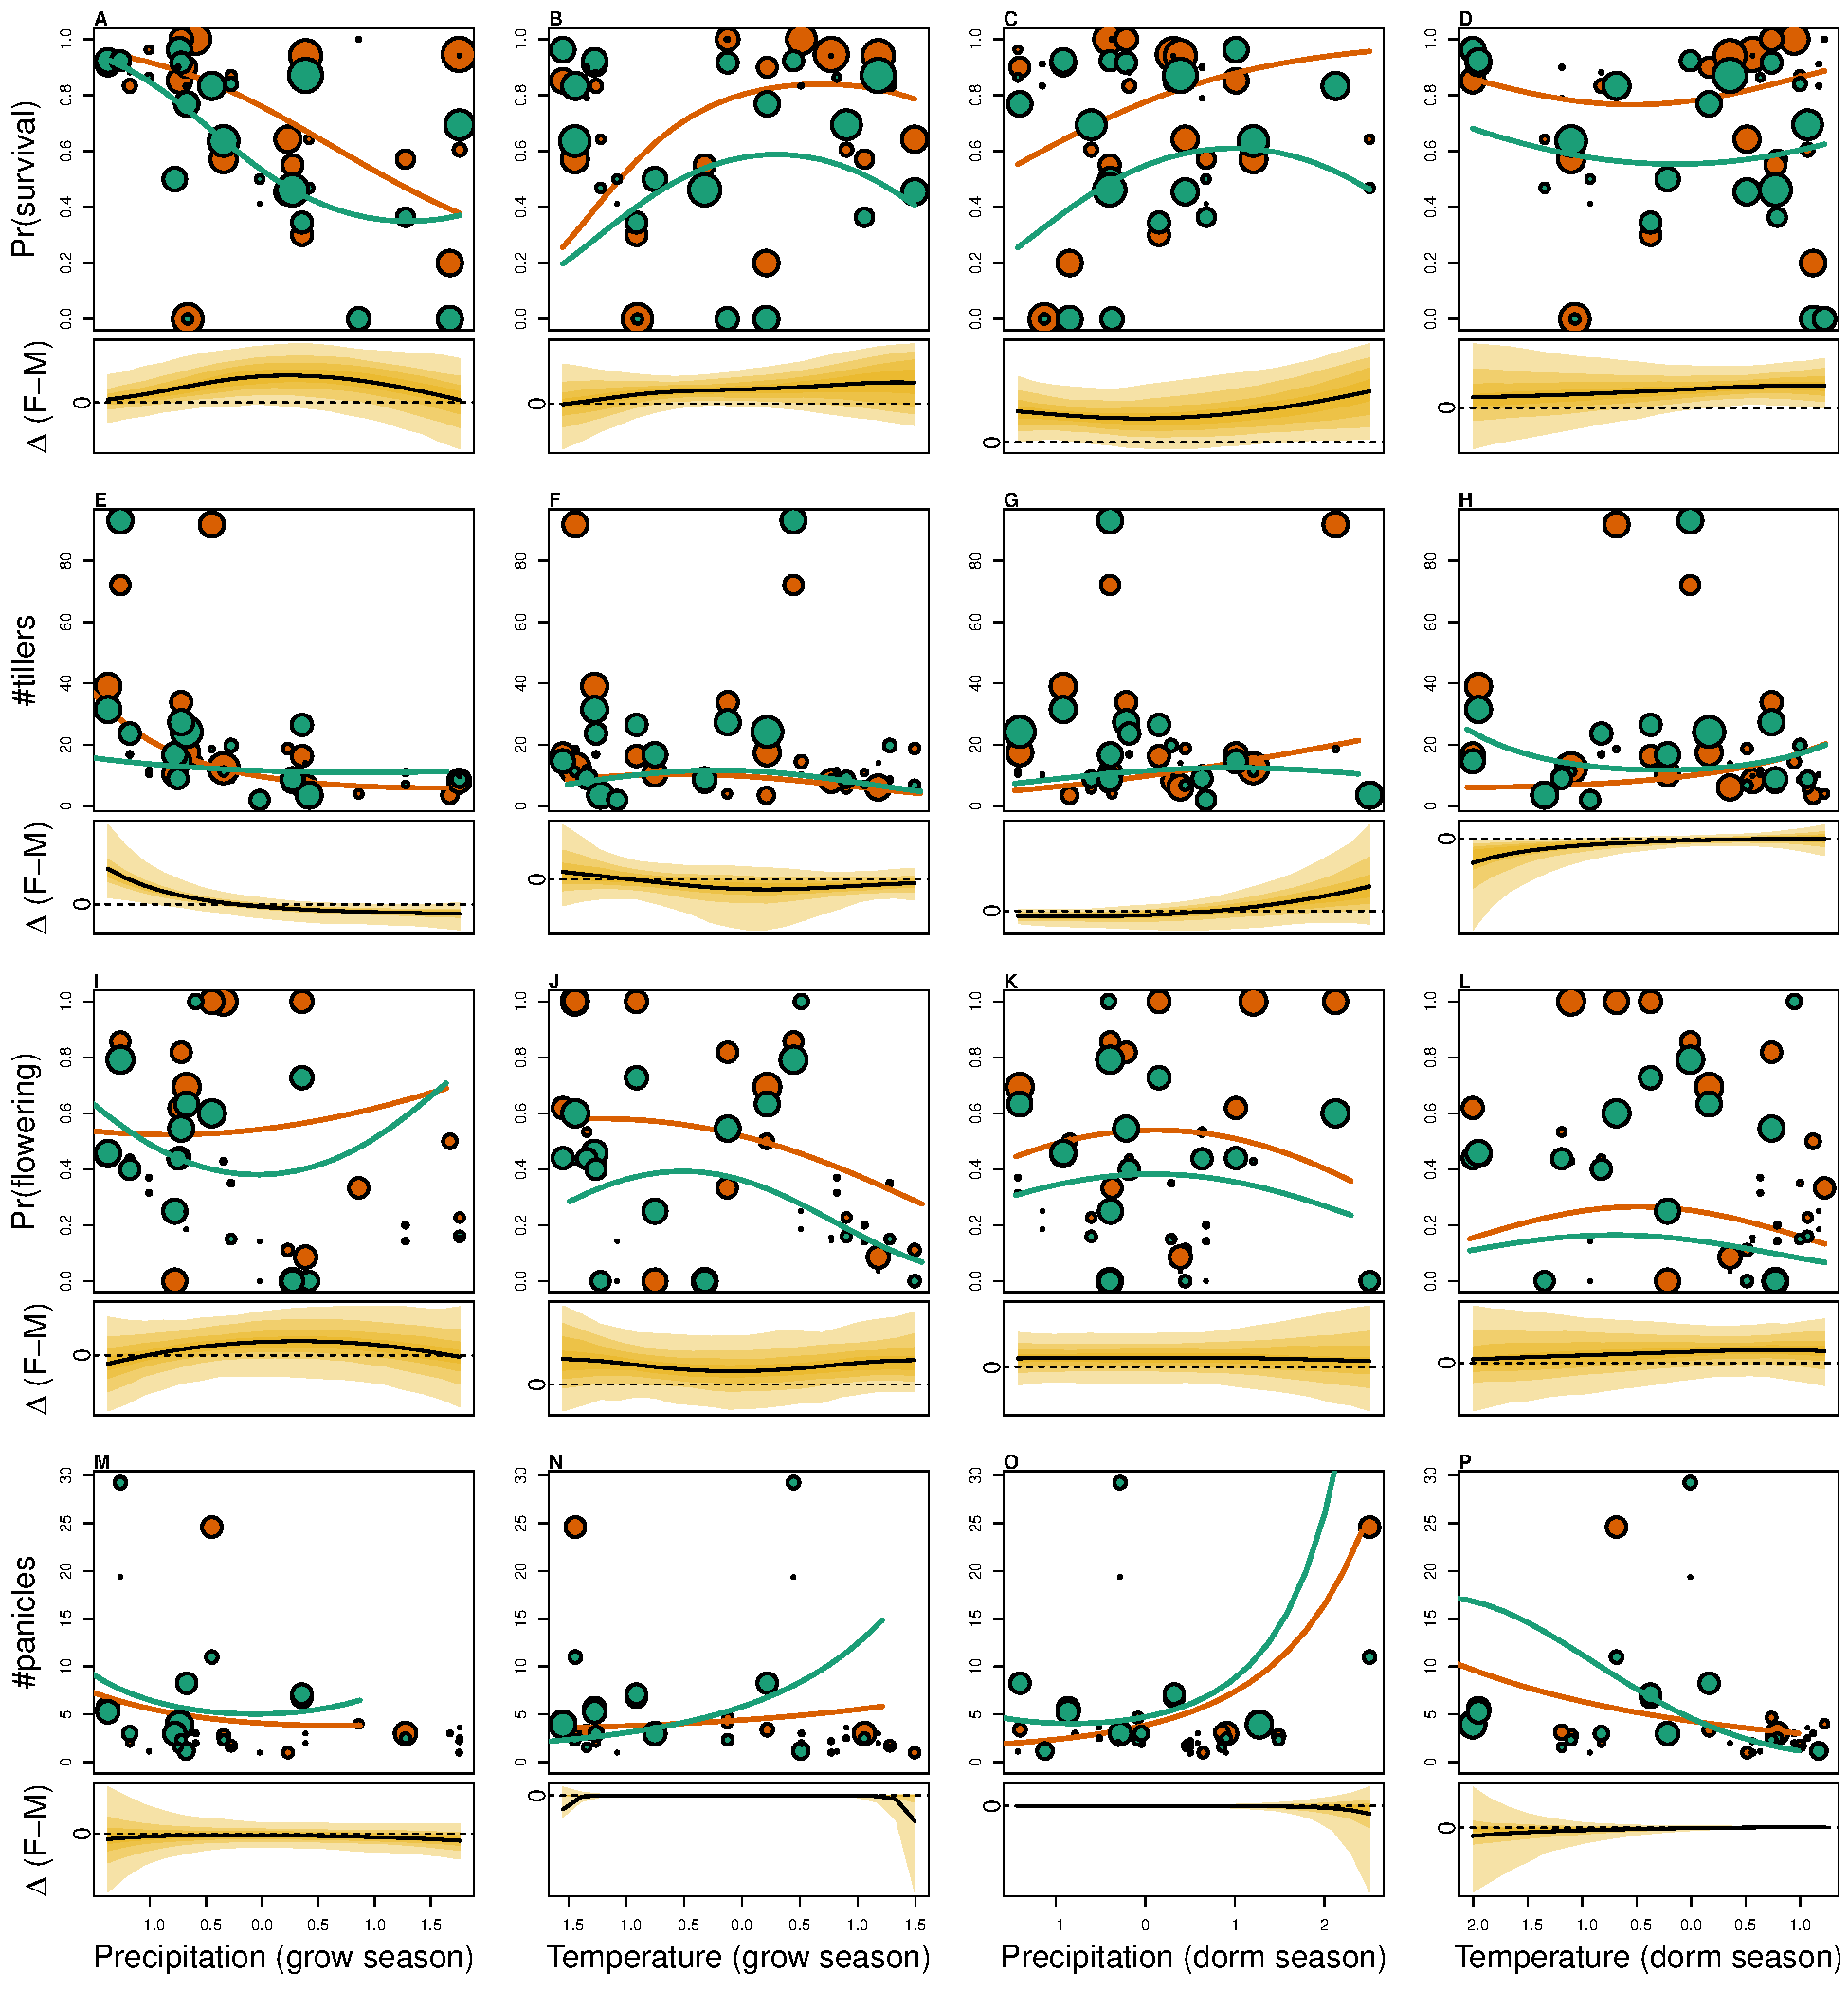
\includegraphics[width=0.80\linewidth]{Figures/vital_rates.pdf}
  \caption{\textbf{Sex specific demographic response to climate across species range}.
  % Vital rates as a function of each climatic variable given 3 others climate variables are constant.
  (A, B, C, D) Probability of survival as a function of precipitation and temperature of the growing and dormant season.
  % (C, D) Probability of survival during the dormant season conditional of climate average during the growing season.
  (E, F, G, H) Change in number of tillers as a function of precipitation and temperature of the growing and dormant season.
  % (F, G) Change in number of tillers during the dormant season conditional of climate average during the growing season.
  (I, J, K, L) Probability of flowering as a function of precipitation and temperature of growing and dormant season.
  % (K, L) Probability of flowering during the dormant season conditional of climate average during the growing season.
  (M, N, O, P) Change in number of panicles as a function of precipitation and temperature of the growing and dormant season.
  % (O, P) Change in number of panicles produced given flowering during the dormant season conditional of climate average during the growing season.
  Points show means by site for females (orange) and males (green). 
  Points sizes are proportional to the sample sizes of the mean and are jittered.
  Lines show fitted statistical models for females (orange) and males (green) based on posterior mean parameter values.
  Lower panels below each data panel show the posterior distribution of the difference between females and males as a function of climate (positive and negative values indicate female and male advantage, respectively); dashed horizontal line shows zero difference.
  % Statistical results are shown in Figure \ref{Sup:Posterior}.
  }
  \label{fig:vital_rates}
  \end{center}
\end{figure}


\subsection*{Female bias in sex-ratio in response to climate climate change}
% There was a significant association between female bias sex-ratio and climate increase. 
Operational-Sex Ratio (proportion of females panicles) increased significantly with an increase of precipitation and temperature of the growing season and precipitation and temperature of dormant season (Figure \ref{Sup:gardens_OSR}, Figure \ref{Sup:PosteriorOSR}). 
Similarly, the proportion of female plants increased with an increase of temperature of growing season and temperature of dormant season (Figure \ref{Sup:gardens_SR} B, D, Figure \ref{Sup:PosteriorSR}).
However, the proportion of female plants did not vary significantly with precipitation of dormant and growing season (Figure \ref{Sup:gardens_SR} A, C). 
Future climate drive to extreme female-biased in \emph{Poa arachnifera} populations (Figure \ref{fig:srprojcmc}, Figure \ref{Sup:osrall}). 

\begin{figure}[H]
  \begin{center}
    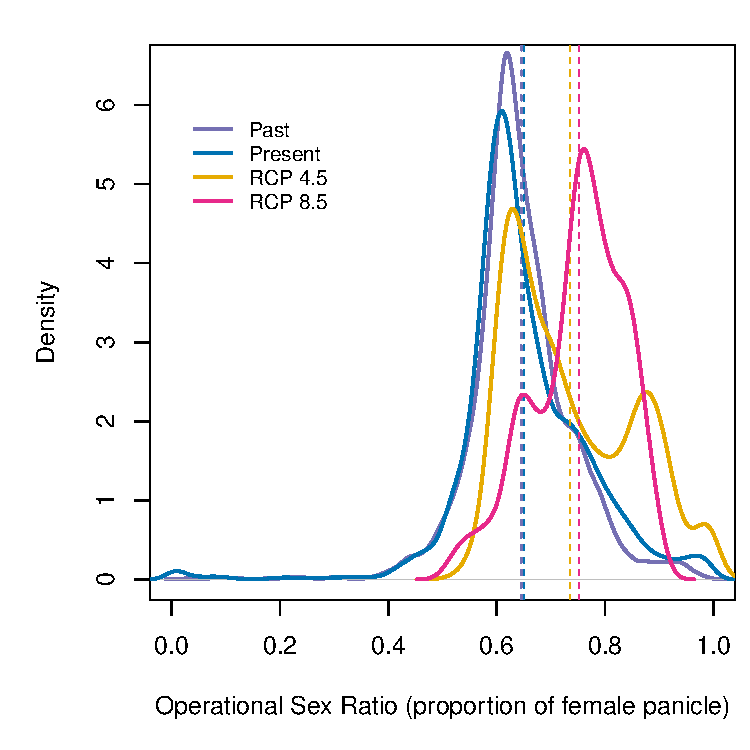
\includegraphics[width=0.8\linewidth]{Figures/POAR_OSR.pdf}
  \caption{Change in Operational Sex Ratio (proportion of female panicule) over time (past, present, future).
  Future projections were based on the CMCC-CM model.
  The mean sex ratio for each time period is shown as vertical dashed line.}
  \label{fig:srprojcmc}
  \end{center}
\end{figure}


\subsection*{Climate change alters population viability}
We estimated population growth rate variation across species range as a function of each climatic variable given the average of the three other climatic variables using two models: \jacob{a female dominant model and a two-sex model}{I have now provided the methods for this contrast.}.
% \tom{Consistent with the effect of climate on the individual vital rate, we found a strong effect of seasonal climate on population fitness (Fig.\ref{fig:lambda}).}{Here and in the preceding figure, I think we need to be more transparent about at what climate values we are purely extrapolating. If I recall correctly, the ``present'' ranges shown in the lambda figure are not the actual range you fit the models over.}
For both models, population growth rate decreased toward high precipitation of growing season (Figure \ref{fig:lambda_LTRE}A).
In contrast population growth rate increased with an increase in precipitation of the dormant season (Figure \ref{fig:lambda_LTRE}C).
Furthermore, population growth rate was maximized between 14 and 17 \degree C and decreased bellow zero beyond 18 \degree C during the growing season (Figure \ref{fig:lambda_LTRE}B).
Similarly population fitness was maximized between 27 and 31 \degree C and decreased bellow zero just beyond 20 \degree C during the dormant season (Figure \ref{fig:lambda_LTRE}D).
% Across species niche population persistence was maximized at higher temperature during the dormant season ( 27 to 31) and intermediate temperature during the growing season (11 to 20).
\jacob{}{I think we should keep this figure. The 2-D niche plots are the better representation of these results, because there are temp*precip interactions that we cannot see here but you can see in the 2-D niche plot. However a model with the 4 predictors together will also give a beter approximation of lambda than the 2D. I added the conditional part in the description of the results. I see the 2D as a way of showing the difference in niche.That said if you really want to remove this I am down you have more experience than me.}

\jacob{We have also detected a strong association between predicted lambda and different ranges of climate (past, present and future).
% However, the magnitude of the effect of future climate on population growth rate was different between emissions scenarios.
Under past climate conditions, population growth rate decreased below one for temperature of the growing season.
Populations will still be viable under moderate gas emission (RCP4.5). 
However high gas emission (RCP8.5) will alter population viability (Figure \ref{fig:lambda_LTRE}B, D).}{I changed how I write the first sentence to remove the "effect of climate on". Again I don't mind removeing the Figure.  }

% \subsection*{Temperature as a driver of population growth rate decline }
Population growth rate was most sensitive to change in temperature of the growing season and temperature of the dormant season (Figure \ref{Sup:LTRE}).
Despite contribution for both sexes, females have a higher contribution to population dynamics than males (Figure \ref{Sup:LTRETemp}; Figure \ref{Sup:LTREppt}).
For both sexes, the reduction of $\lambda$ for high value of temperature  (dormant and growing season) was driven by a reduction of survival rate, growth rate, and a reduction in number of panicles (Figure \ref{fig:lambda_LTRE}F, H, G, L).
However, the change of population growth rate for high value of precipitation was not driven by change in vital rates.

\begin{figure}[H]
  \begin{center}
    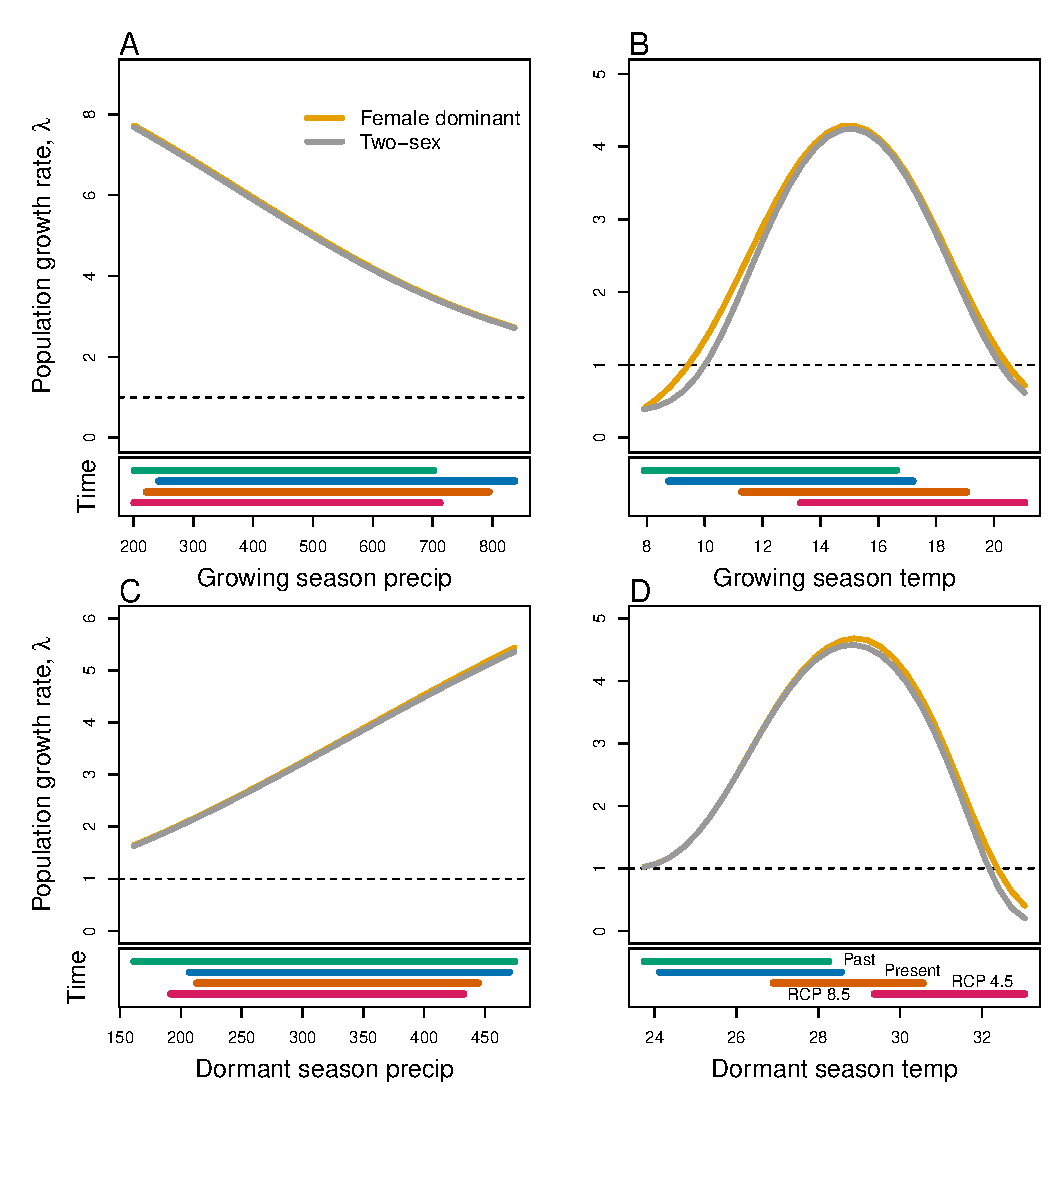
\includegraphics[width=1\linewidth]{Figures/lambda_past_present_future.pdf}
  \caption{\textbf{Predicted population growth rate ($\lambda$) in different ranges of climate}.
(A) Precipitation of the growing season, (B) Temperature of the growing season, (C) Precipitation of the dormant season, (D) Temperature of the dormant season.
The grey curve shows prediction by the two-sex matrix projection model that incorporates sex- specific demographic responses to climate with sex ratio dependent seed fertilization.
The orange curve represents the prediction by the female dominant matrix projection model.
The dashed horizontal line indicates the limit of population viability ($\lambda$ = 1).
Lower panels below each data panel shows  ranges of climate values for different time period (past climate, present and future climates).
For future climate, we show a Representation Concentration Pathways (RCP) 4.5 and 8.5. Values of ($\lambda$) are derived from the mean climate variables across 4 GCMs (MIROC5, ACCESS1-3, CESM1-BGC, CMCC-CM).
% Life table response experiment decomposition of the sensitivity of $\lambda$ to seasonal climate into additive vital rate contributions of males and females based on posterior mean parameter estimates.
%  (A) Temperature of growing season (contribution of female), (B) Temperature of growing season (contribution of male),  (C) Temperature of dormant season (contribution of female) and (D) Temperature of dormant season (contribution of male).
}
  \label{fig:lambda_LTRE}
  \end{center}
\end{figure}



\subsection*{Climatic change induces niche and range shifts}
% Female dominant model and the two-sex models predict that populations of \emph{Poa arachnifera} were more likely to be viable (Pr ($\lambda$ > 1)) at intermediate values of temperature of dormant and growing season (Fig. \ref{fig:niche}; Fig. \ref{Sup:lambda2D} B, D).
% For both models, population viability decreased toward high precipitation of growing season and low values of precipitation of the dormant season (Fig. \ref{fig:niche}; Fig. \ref{Sup:lambda2D} A, B).
% The spatio-temporal variation of population viability was driven by variation in vital rate for both male and female individuals (Fig. \ref{Sup:LTRETemp}, Fig. \ref{Sup:LTREppt}). 
Female dominant model and  two-sex models predicts a niche shift in \emph{Poa arachnifera} populations (Figure \ref{fig:niche}). 
% However the female dominant model under estimated the impact of climate effect particularly for location of the range with higher value of temperature and precipitation (Fig. \ref{fig:niche} E,F). 
%  
However, the female dominant model underestimated the magnitude of niche shifts (Figure \ref{fig:niche}E, F; -0.16[-0.29,-0.03]).
% That niche shift was probably due to high sensitivity of population viability to temperature of growing season season and dormant season (Fig. \ref{Sup:LTRE}).
Female dominant model and the two-sex models agree that viable populations of \emph{P. arichnifera} were only predicted at the center of the range for current climatic conditions (Figure \ref{fig:geoprojacc}).
Although \emph{P. arichnifera} was predicted to have suitable habitats in the center of the range under current climate, global  warming is projected to reduce much of these suitable habitats (Figure \ref{fig:geoprojacc}). 
If the species is able to disperse far and if there is no physical barriers, most of the current suitable habitats will move toward the Northern range edge as a results of niche shifts. 
Niche shift underestimation by the female dominant model led to a geographic range underestimation by the female dominant model.  



\begin{figure}[H]
  \begin{center}
    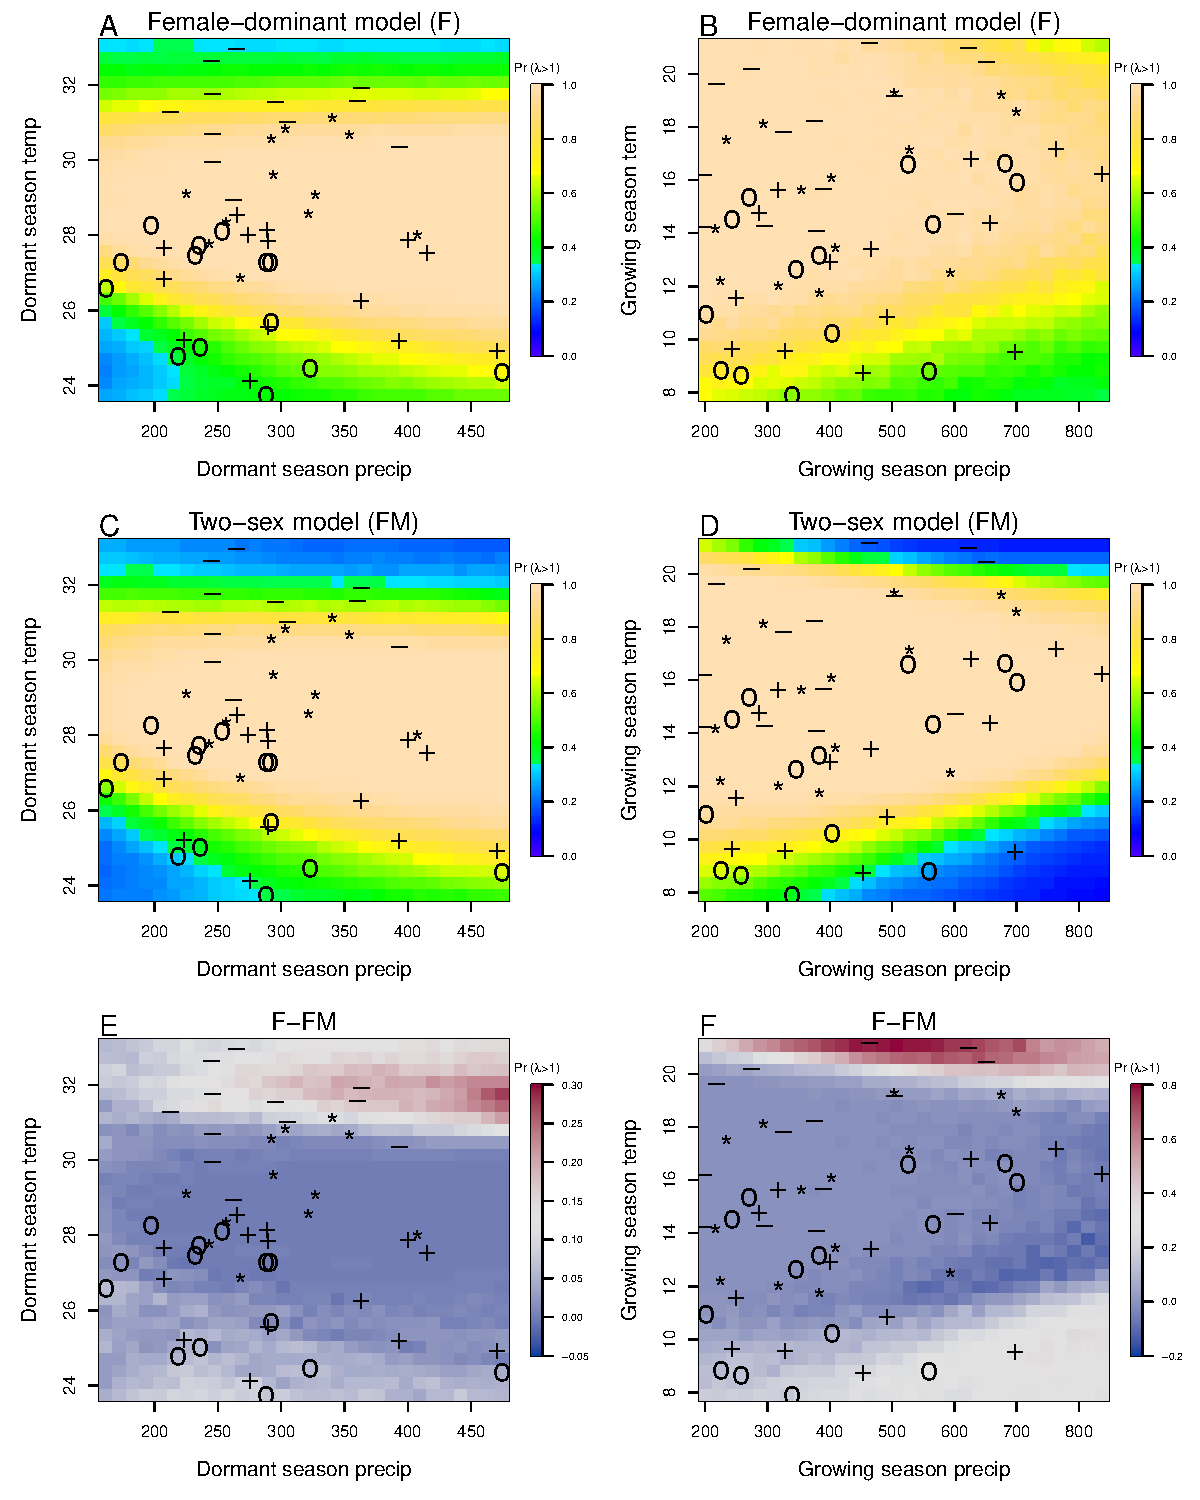
\includegraphics[width=0.95\linewidth]{Figures/niche_dormant_growing.pdf}
  \caption{\textbf{A two‐dimensional representation of the predicted niche shift over time (past, present and future climate conditions)}. 
  Contours on the first four panels show predicted probabilities of self- sustaining populations, Pr ($\lambda > 1$) conditional on precipitation and temperature of the dormant and growing season.
 % (A) Niche ( Pr ($\lambda$ > 1)) of dormant season for female dominant model, (B) Niche of growing season for female dominant model.
 % (C) Niche ( Pr ($\lambda$ > 1))of dormant season for the two sex model, (B) Niche of growing season for the two-sex model.
 The last two panels show difference in niche estimation between the female dominant model and the two-sex model for each season.
  "\begin{normalsize}\textbf{o}\end{normalsize}": Past, "\begin{normalsize}\textbf{+}\end{normalsize}": Current,"\begin{large}\textbf{*}\end{large}": RCP 4.5,"\begin{tiny}$\blacksquare$\end{tiny}": RCP 8.5.}
  \label{fig:niche}
  \end{center}
\end{figure}

\begin{figure}[H]
  \begin{center}
    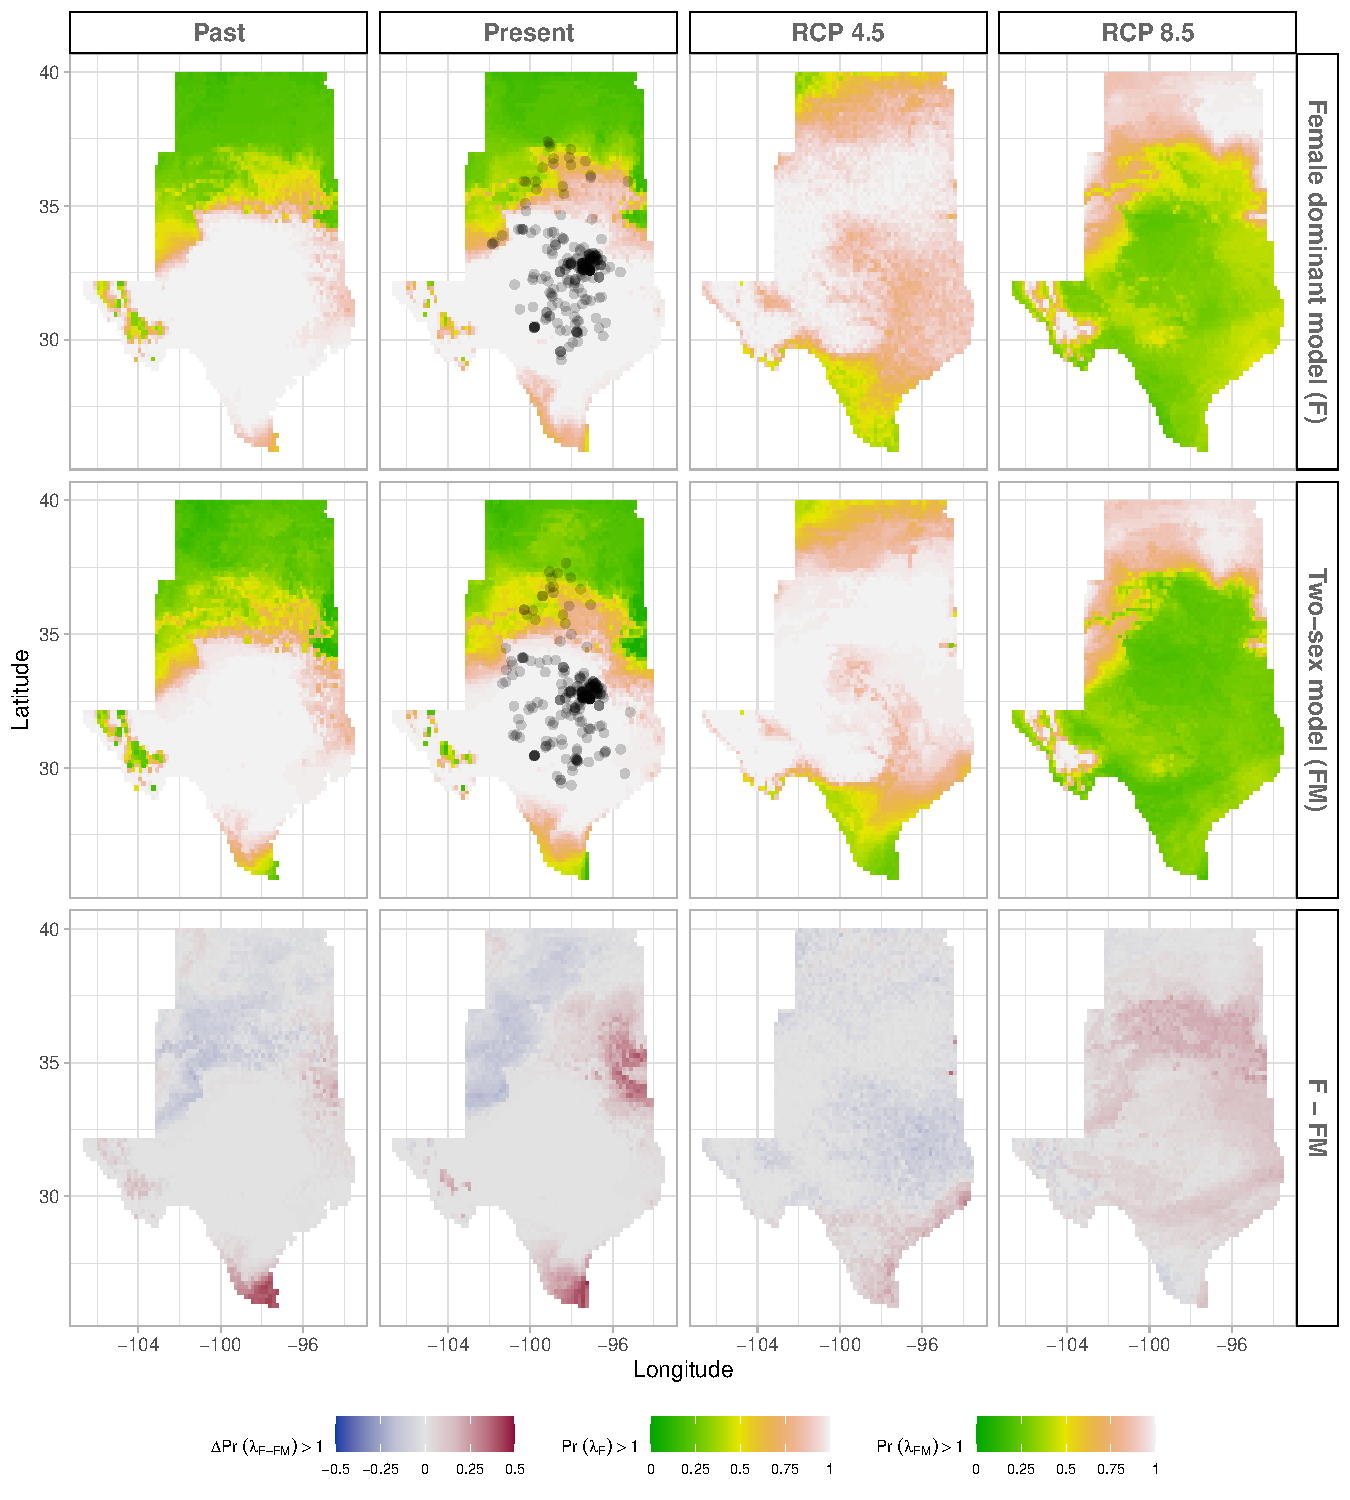
\includegraphics[width=0.99\linewidth]{Figures/Fig_geoPrlambdacmc.pdf}
  \caption{ \textbf{Climate change favors range shift towards north edge.}
  (A) Past, (B) Current, (C and D) Future predicted range shift based on the predicted probabilities of self- sustaining populations, Pr ($\lambda > 1$), using the two-sex model that incorporates sex- specific demographic responses to climate with sex ratio dependent seed fertilization.
  (E) Past, (F) Current, (G and F) Future  predicted range shift based on the predicted probabilities of self- sustaining populations, Pr ($\lambda > 1$), using the female dominant model.
  Future projections were based on the CMCC-CM model.
  The black dots on panel B and F indicate all known presence points collected from GBIF from 1990 to 2019, which corresponds to the current condition in our prediction. 
  The occurrences of GBIFs are distributed in with higher population fitness habitat Pr ($\lambda$ > 1) , confirming that our study approach can reasonably predict range shifts. }
  \label{fig:geoprojacc}
  \end{center}
\end{figure}


\section*{Discussion}
\jacob{}{This is my new proposition regarding the discussion}Dioecioius species make up a large fraction of Earth's biodiversity -- most animals and many plants -- yet we have little knowledge about how skewness in sex ratio will affect population viability and range shifts of dioecious species under climate change.
We used three years of demographic data collected common garden experiments across climatic gradient to forecast for the first time the impact of climate change on dioecious species.
% Our models captures a certain range of demographic and environmental variability (Figure \ref{Sup:lambda2sex}).
Our future projections require extrapolation to warmer or colder conditions than observed in our experiment and subsequently should be interpreted with caution \citep{chen2024influence}.
Despite all these limitations, the qualitative implications of the response of our study species to increase temperature (dormant and growing season) seems consistent across all GCMs (Figure \ref{Sup:geoprojces}, Figure \ref{Sup:geoprojcmc}, Figure \ref{Sup:geoprojmiroc}).  
% Most of the suitable areas move toward the North, beyond the current range in response to climate change.
% \tom{Climate change will affect population growth rate primarily through the response of female which is more sensitive to climate change \citep{miller2022two}.}{This paper says the opposite.}
% \tom{Males also have a significant contribution to population growth rate particularly for temperature. }{I do not know what this is saying.}
Three general patterns emerged from our analysis of range-wide common garden experiments and sex-structured, climate-explicit demographic models.
First, our Bayesian mixed effect model suggests a sex specific demographic response to climate change that lead to higher proportion of female as climate increase.
Second, climate change favors a northern range shifts in suitable  habitats. 
Third, the female dominant model (model that does not account for sex structure) overestimates species niche and range shifts.

There was a female demographic advantage leading to a female biased in response to climate change in \emph{Poa arachnifera} populations.
% The female demographic advantage is not unique to our study system and has been observed in several dioecious species \citep{welbergen2008climate,zhao2012sex,sasaki2019complex}.
The extreme female-bias in response to climate change contrast with  previous studies suggesting that an increase in male frequency in response in climate change \citep{petry2016sex,hultine2016climate}.
Two mechanisms could explain the observed demographic advantage of females over males for survival and flowering and the opposite for growth and number of panicles.
The trade-off between fitness traits (survival, growth and fertility) due to resource limitation and the pollination mode of our study species (wind pollinated) could explain such a result \citep{cipollini1994sexual,freeman1976differential}.
For most species, the cost of reproduction is often higher for females than males due to the requirement to develop seeds and fruits \citep{hultine2016climate}. 
However, several studies reported a higher cost of reproduction for males in wind pollinated species due to the larger amounts of pollen they produce \citep{burli2022environmental,cipollini1994sexual,bruijning2017surviving,field2013comparative}.

% \tom{Under current conditions, most populations across the range are viable.}{I don't think this statement is well-supported. We don't have any data from natural populations.}
% This result could be explained by two hypotheses.
% First, demographic compensation whereby an increase of one vital rate is coupled with a decrease of another vital rate could explain viable populations in harsh conditions at the range edge \citep{doak2010demographic,villellas2015demographic,nomoto2021drivers}. 
% In our system, a decrease in fertility and survival rate was counterbalanced by an increase in flowering rate, \tom{preventing the population growth rate from declining even at range edge}{Not sure I follow this - if lambda was not declining it would not be a range edge} \tom{during the dormant season}{Population growth rate is an annual measure, it does not refer to any season. I think what you mean here is that dormant season weather can affect population growth rate.}.
% Second, local adaptation at the edge of the range could explain the viable populations throughout the range \citep{miller2022two}. 
% \tom{Our study was based on a common garden experiment; therefore, individuals planted in climatic conditions that are similar to their source populations climatic conditions were less impacted by stressful environmental conditions.}{This statement lacks evidence.}
% \tom{An important question to ask is: what is the role of local adaptation in buffering species response against climate change.
% Unfortunately, our model does not shed light on that question.
% Adding another predictor to our complex model would have lead to overfitting. 
% Therefore, the role of local adaptation in mitigating population response to climate should be the next step in forecasting species response to climate. }{I don't think this is a very effective use of the Discussion. If you want to address local adaptation maybe that can go in an appendix. I don't actually understand the point of this paragraph but maybe I am not understanding something.}

% Our LTRE analysis reveals that a small change in temperature of the growing and dormant season could have a larger  impact on population viability.
% % This results corroborated with other studies and suggest that projected future climate will affect population viability \citep{reed2021climate}. 
% Temperature can impact plant populations through different mechanisms. 
% Increasing temperature could increase evaporative demand, affect plant phenology \citep{mclean2016predicting,sherry2007divergence,iler2019reproductive}, and germination rate \citep{reed2021climate}.
% % In the  growing season, when the temperature is high, the effect on the water balance should be strong .
% The potential for temperature to influence these different processes changes seasonally \citep{konapala2020climate}.
% For example, studies suggested that species that are active during the growing season such as cool grass species can have delayed phenology in response to global warming, particularly if temperatures rise above their physiological tolerances \citep{cleland2007shifting,williams2015life}. 
% In addition, high temperature during the growing season by affecting pollen viability, fertilization could affect seed formation and germination \citep{hatfield2015temperature,sletvold2015climate}. 
% % Because our study species was sensitive to temperatures in the growing season, the former mechanism deserve further attention.
% \tom{Temperature also affected operational sex ratio (OSR) (Fig.XX). 
% That variation in OSR could affect population growth rate by altering females’ fitness \citep{petry2016sex,knight2005pollen,haridas2014frequency}. }{These results need to be beter developed because they underlie all the other results. And again, the only way you can get an effect on temperature on OSR is if there were sex-specific responses to climate, but you way there were none.}

Our results suggest that climate change will alter population at the center of the range and drive a northern range shifts. 
This impact of climate change on the species current niche could be explained by the increase of temperature over the next years.
Small change in temperature of the growing and dormant season have a larger impact on population viability.
Temperature can impact plant populations through different mechanisms.
Increasing temperature could increase evaporative demand, affect plant phenology \citep{mclean2016predicting,sherry2007divergence,iler2019reproductive}, and germination rate \citep{reed2021climate}.
% In the  growing season, when the temperature is high, the effect on the water balance should be strong .
The potential for temperature to influence these different processes changes seasonally \citep{konapala2020climate}.
For example, studies suggested that species that are active during the growing season such as cool grass species can have delayed phenology in response to global warming, particularly if temperatures rise above their physiological tolerances \citep{cleland2007shifting, williams2015life}.
In addition, high temperature during the growing season by affecting pollen viability, fertilization could affect seed formation and germination \citep{hatfield2015temperature,sletvold2015climate}.
Pollen dispersal may allow plants to resist climate change because pollen dispersal may provide the local genetic diversity necessary to adapt at the leading edge of the population \citep{kremer2012long,corlett2013will,duputie2012genetic}.
Since wind pollination is most effective at short distances, it is most often found in plant species growing at high density such as our study species, it is less likely that dispersal limitation  affect niche shift in our study system.
Difference in non-climatic factors such as soil, or biotic interactions could also explain decline in population growth rate as an indirect effects of increase in temperature \citep{alexander2015novel,schultz2022climate}.
For example, climate change could increase the strength of species competition and thereby constrain our study species  to a narrower realized niche \citep{pulliam2000relationship,aguilee2016pollen}.
% Future studies should studies should investigate how biotic factors drive range limits. 

We found evidence of underestimation of the impact of climatic change on population dynamics by the female dominant model and implication for such an underestimation on conservation actions for dioecious species.
The underestimation of the impact of climatic change on population dynamics by the female dominant model makes sense given the sex specific response to climatic change. 
\emph{Poa arachnifera} populations will be female biased in response to climate change.
That extreme female-bias could affect population growth rate by altering males’ fitness with reduction on mate availability given that females individuals have a demographic advantage over males \citep{knight2005pollen,haridas2014frequency}.
Further, our work suggest that population viability is sensitive to climate under current  and future conditions.
This is key because most conservation actions are design from  data on current responses to climate, rather than future response to climate \citep{sletvold2013climate}.
Since the role of male is not negligible in accuraltly predicting dioecious species response to climate change, management strategies that focus on both sexes would be effective and will enhance our understanding of dioecious species response to global warming.

\section*{Conclusion}
We have investigated the potential consequence of skewness in sex ratio on population dynamics and range shift in the context of climate change using the Texas bluegrass. 
We found extreme female -biased in response to climate change. 
The effect of female biased will induce range shifts to the northern edge of the species current range by limiting mate availability.
Beyond, our study case, our results also suggest that tracking only one sex could lead to an underestimation of the effect of climate change on population dynamics. 
Our work  provides also a framework for predicting the impact of global warming on population dynamics using the probability of population to self-sustain. 

\section*{Acknowledgements}
This research was supported by National Science Foundation Division of Environmental Biology awards 1543651 and 1754468 and by the Rice University Faculty Initiatives Fund.



\newpage
\bibliographystyle{apalike}
\bibliography{Forecasting}
%--------------------------------------------------------------------
\newpage
\clearpage 
\setcounter{equation}{0}
\setcounter{figure}{0}
\setcounter{section}{0}
\setcounter{table}{0}
\renewcommand{\theequation}{S.\arabic{equation}}
\renewcommand{\thetable}{S-\arabic{table}}
\renewcommand{\thefigure}{S-\arabic{figure}}
\renewcommand{\thesection}{S.\arabic{section}}

\centerline{\Large{\textbf{Supporting Information}}}

\section {Supporting Figures}

\begin{figure}[H]
		\centering
		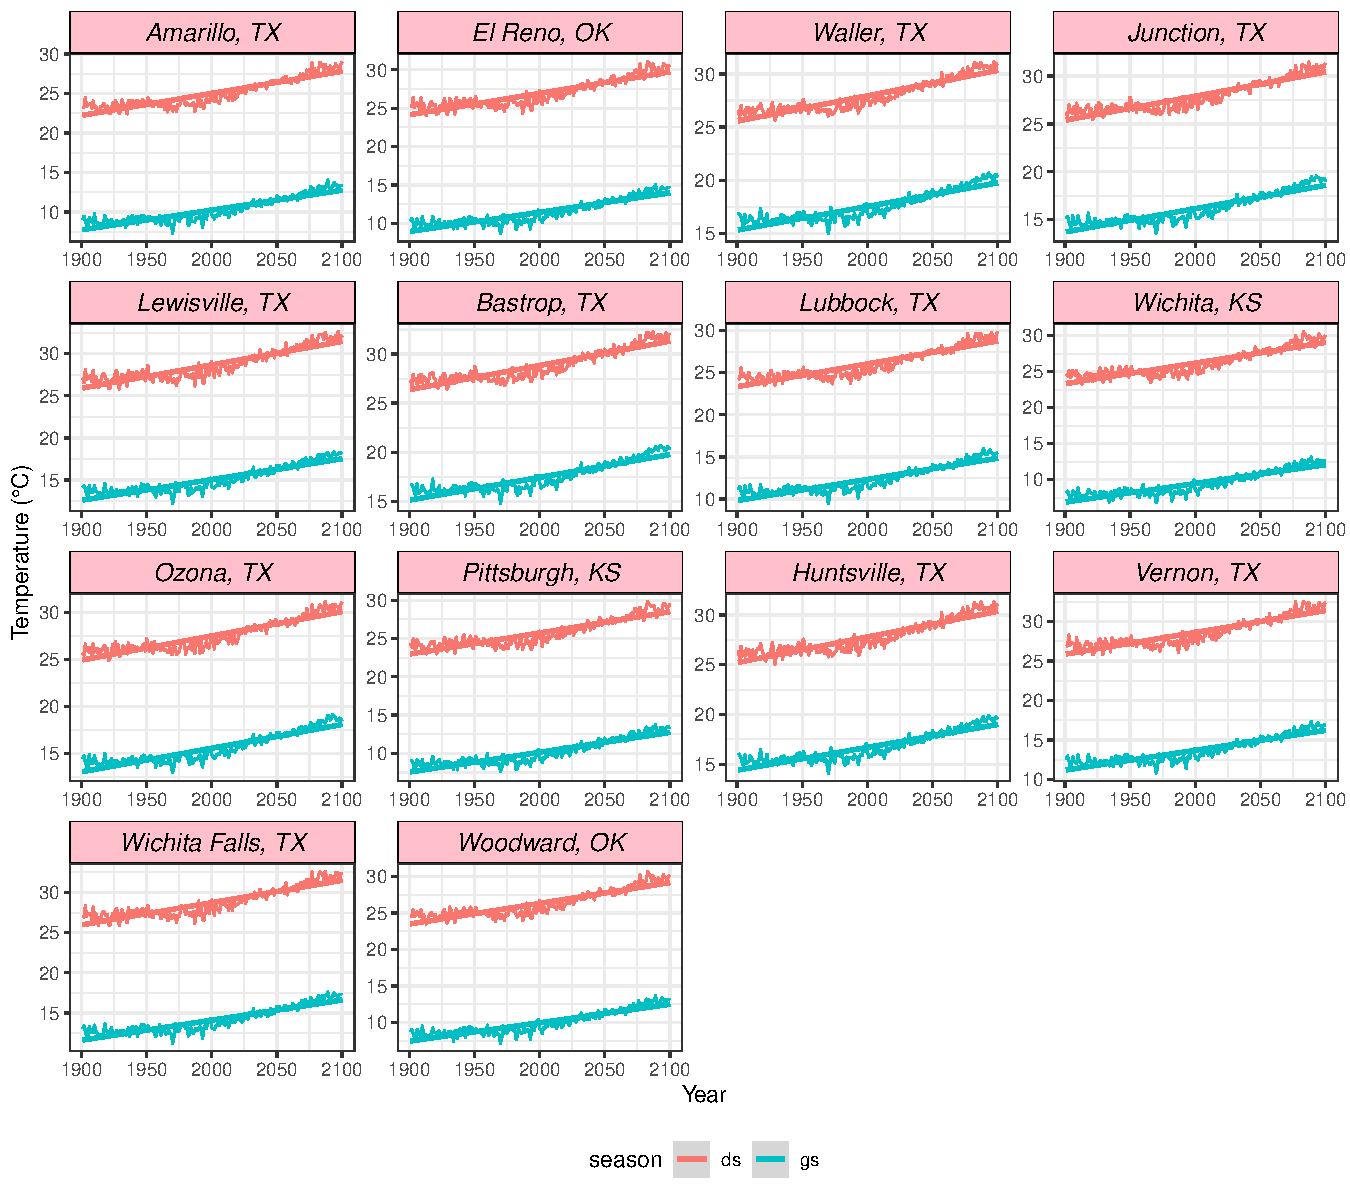
\includegraphics[width=0.95\linewidth]{Figures/fig_tas_past_present_future.pdf}
		\caption{Temperature variation across the study sites from 1990 to 2100,
		ds: Dormant season, dg: Growing season.}
		\label{Sup:temp_variation}
\end{figure}

\begin{figure}[H]
		\centering
		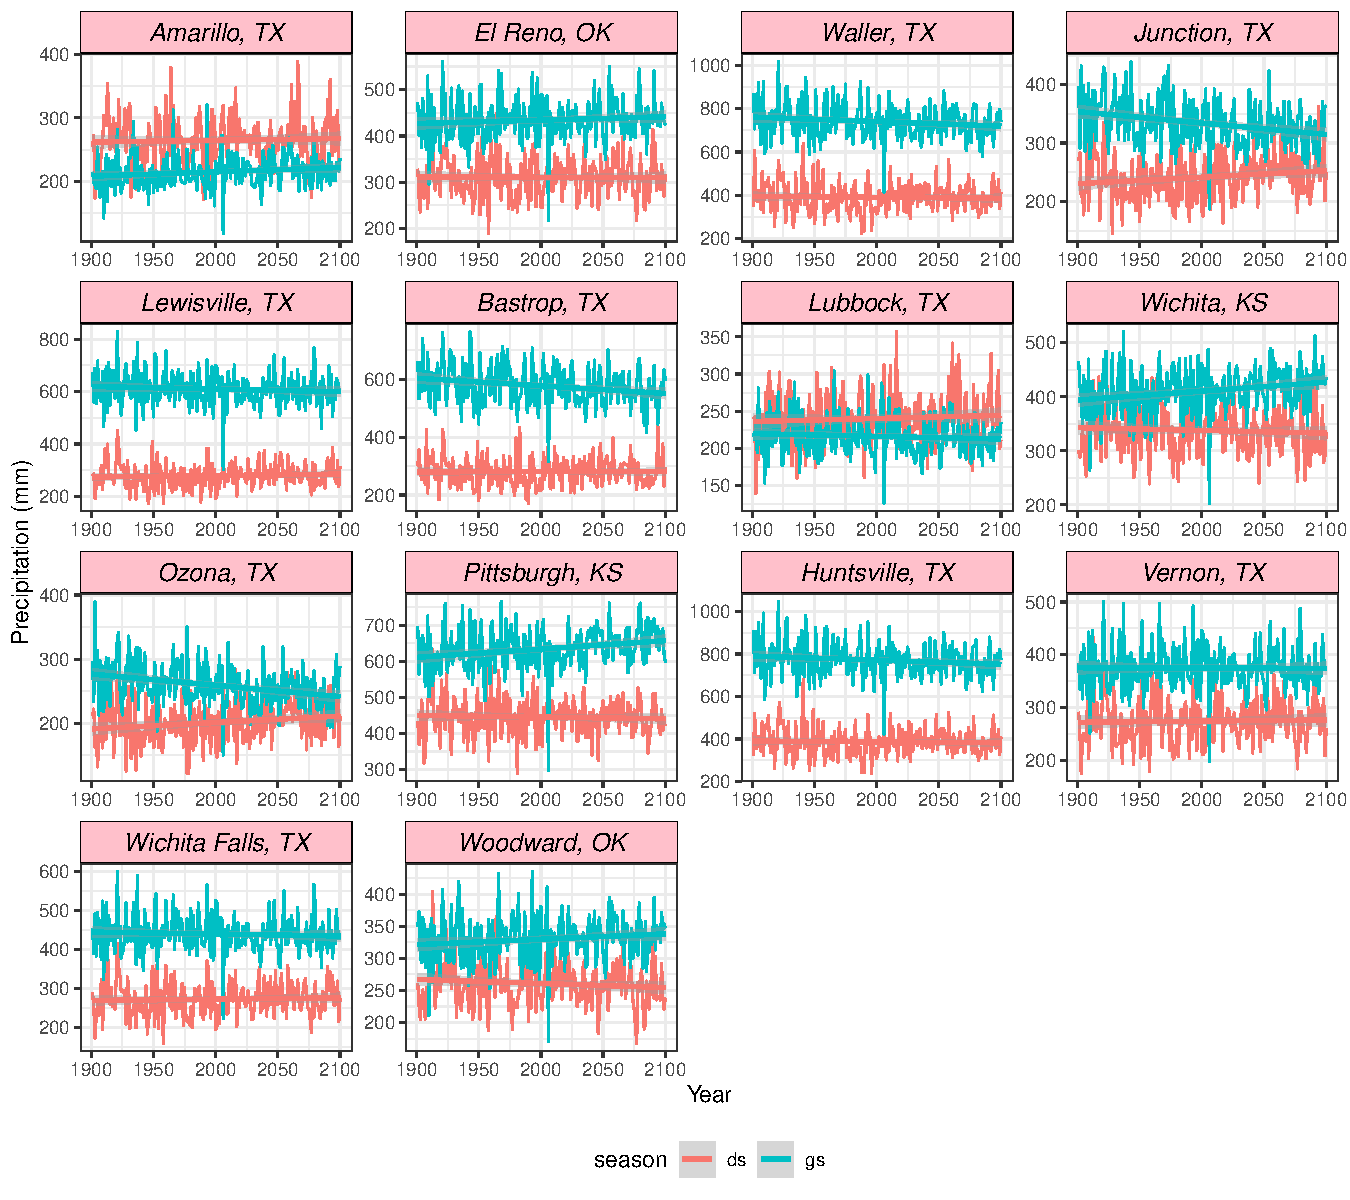
\includegraphics[width=0.95\linewidth]{Figures/fig_pr_past_present_future.pdf}
		\caption{Precipitation variation across the study sites from 1990 to 2100.
		ds: Dormant season, dg: Growing season.}
		\label{Sup:pr_variation}
\end{figure}

\begin{figure}[H]
		\centering
		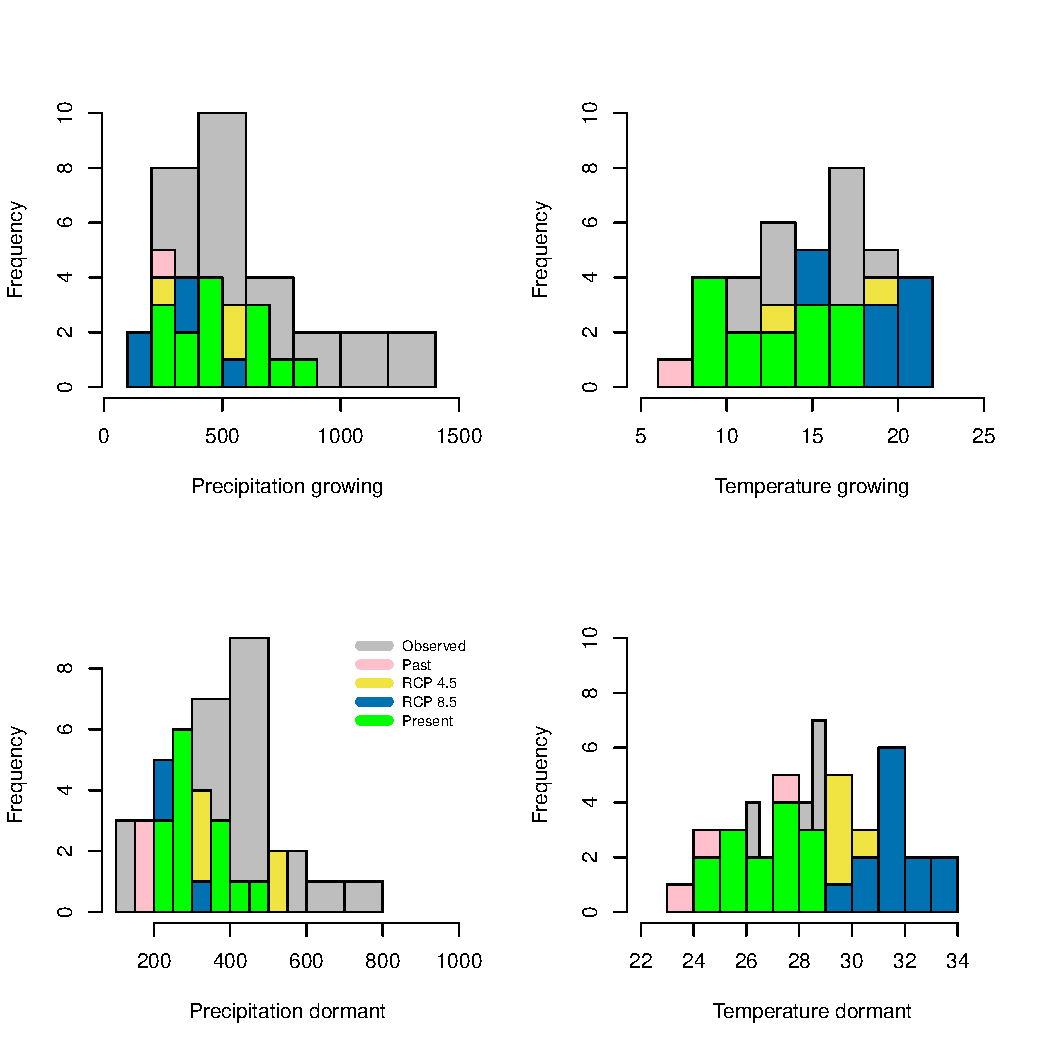
\includegraphics[width=0.95\linewidth]{Figures/MIROC.pdf}
		\caption{Past, Observed, present and future (MIROC Model) climate data across the study area.}
		\label{Sup:projectionMIROC}
\end{figure}

\begin{figure}[H]
		\centering
		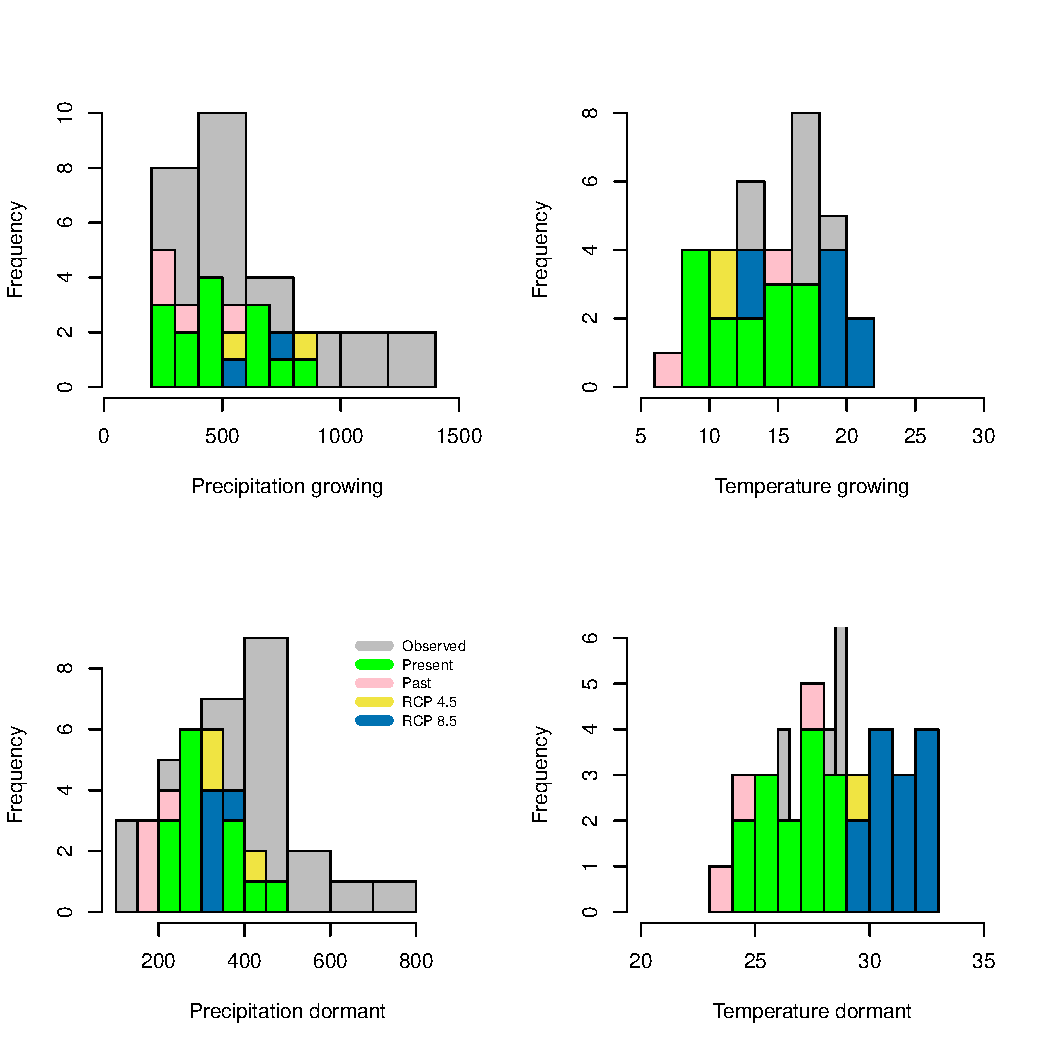
\includegraphics[width=0.99\linewidth]{Figures/ACCESS.pdf}
		\caption{Past, Observed, present and future (ACCESS Model) climate data across the study area.}
		\label{Sup:projectionACCESS}
\end{figure}

\begin{figure}[H]
		\centering
		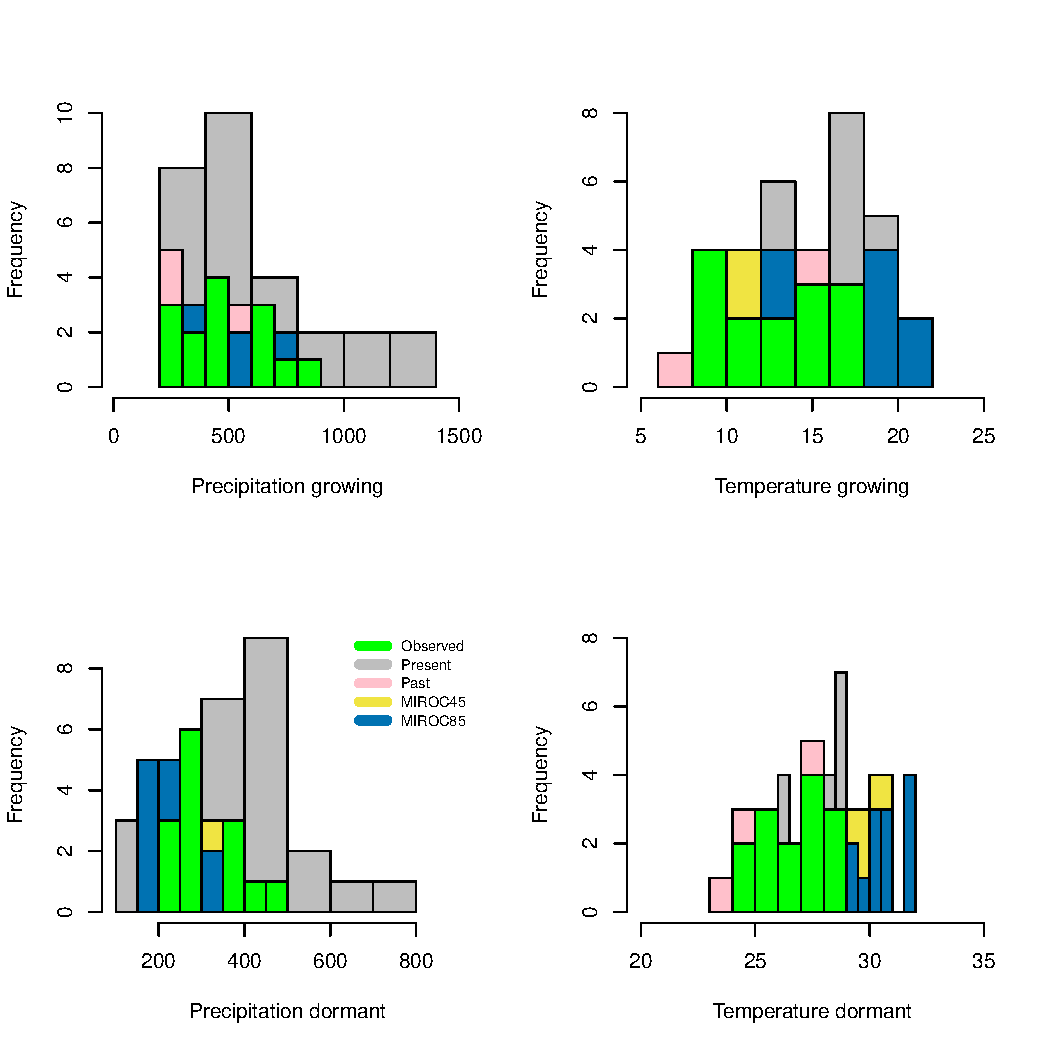
\includegraphics[width=0.99\linewidth]{Figures/CESM1.pdf}
		\caption{Past, Observed, present and future (CESM1 Model) climate data across the study area.}
		\label{Sup:projectionCESM1}
\end{figure}

\begin{figure}[H]
		\centering
		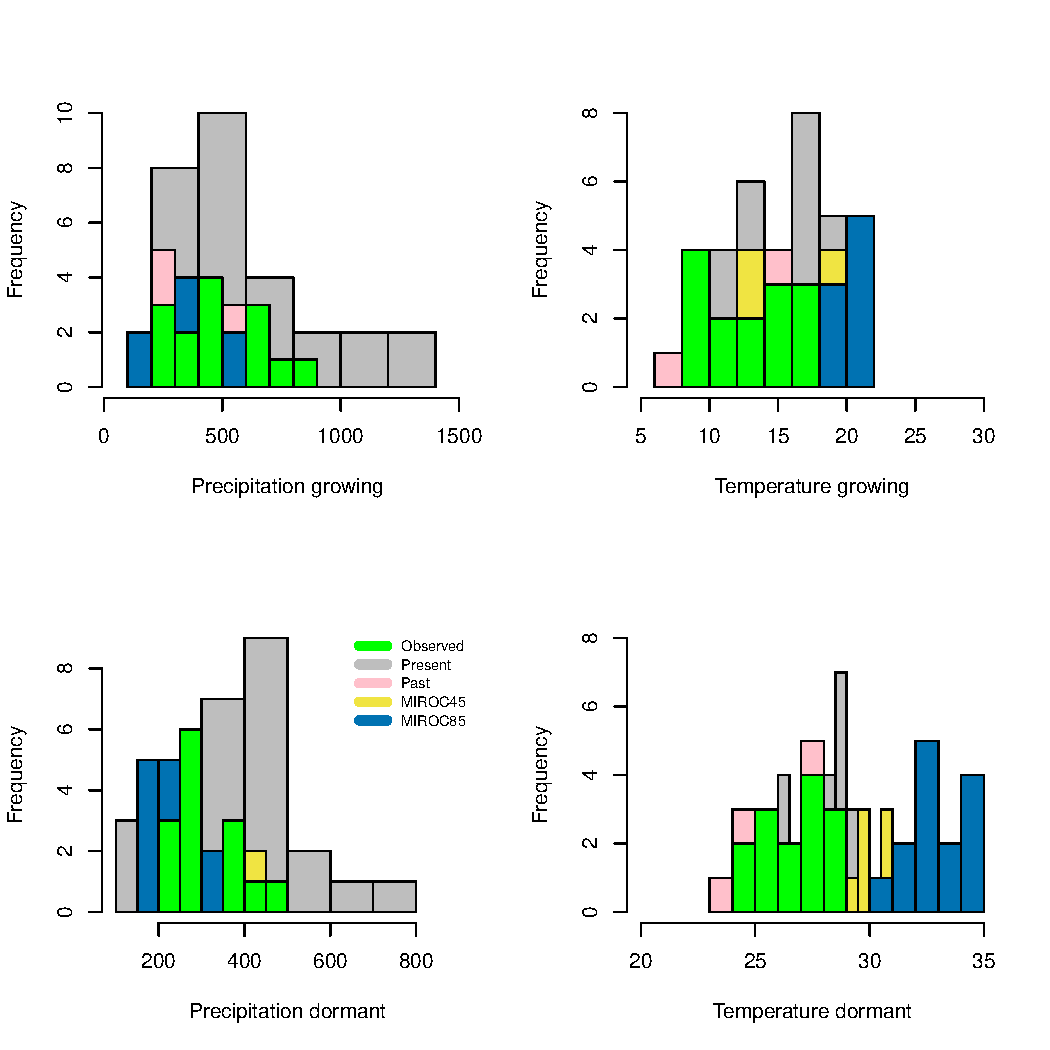
\includegraphics[width=0.99\linewidth]{Figures/CMCC.pdf}
		\caption{Past, Observed, present and future (CMCC Model) climate data across the study area.}
		\label{Sup:projectionCMCC}
\end{figure}

\begin{figure}[H]
		\centering
		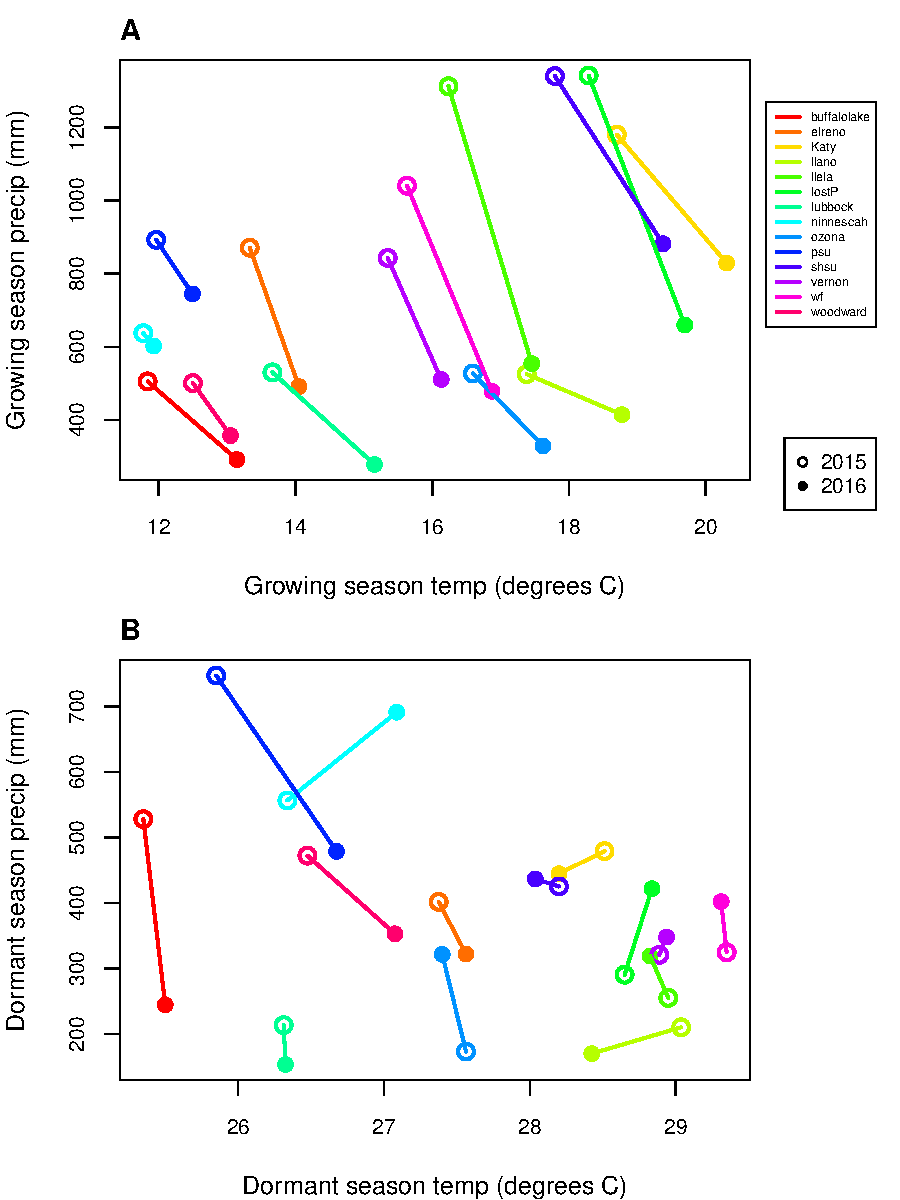
\includegraphics[width=0.959\linewidth]{Figures/site_year_weather.pdf}
		\caption{Climate variation across the study sites during the monitoring period.}
		\label{Sup:climate_variation}
\end{figure}

% \begin{figure}[H]
% 		\centering
% 		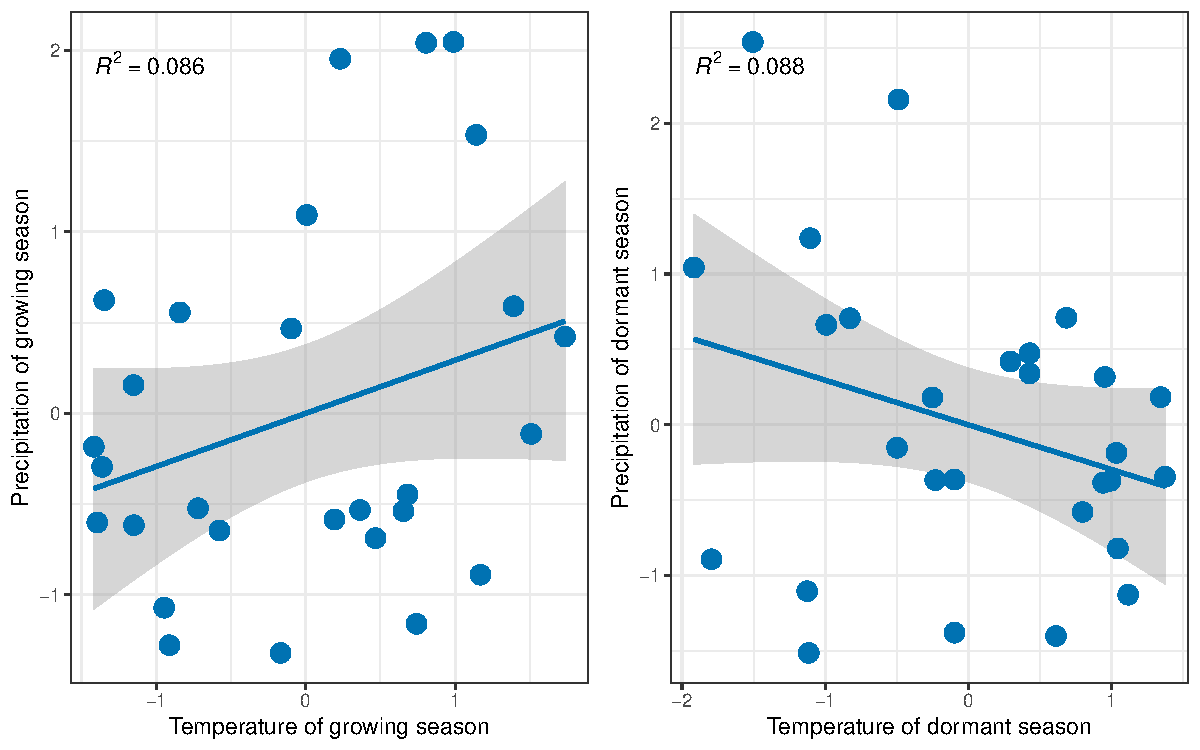
\includegraphics[width=0.95\linewidth]{Figures/Varianceexplained.pdf}
% 		\caption{Relation between precipitation and temperature for each season (growing and dormant). $R^2$ indicates the value of proportion of explained variance between the temperature and precipitation}
% 		\label{Sup:Correlation}
% \end{figure}
	
\begin{figure}[H]
		\centering
		\includegraphics[width=0.75\linewidth]{Figures/PPC.pdf}
		\caption{Posterior predictive checks. Consistency between real data and simulated values suggests that the fitted vital rate models accurately describes the data. Graph shows density curves for the observed data (light orange ) along with the simulated values (dark orange).}
		\label{Sup:PPC}
	\end{figure}

\begin{figure}[H]
		\centering
		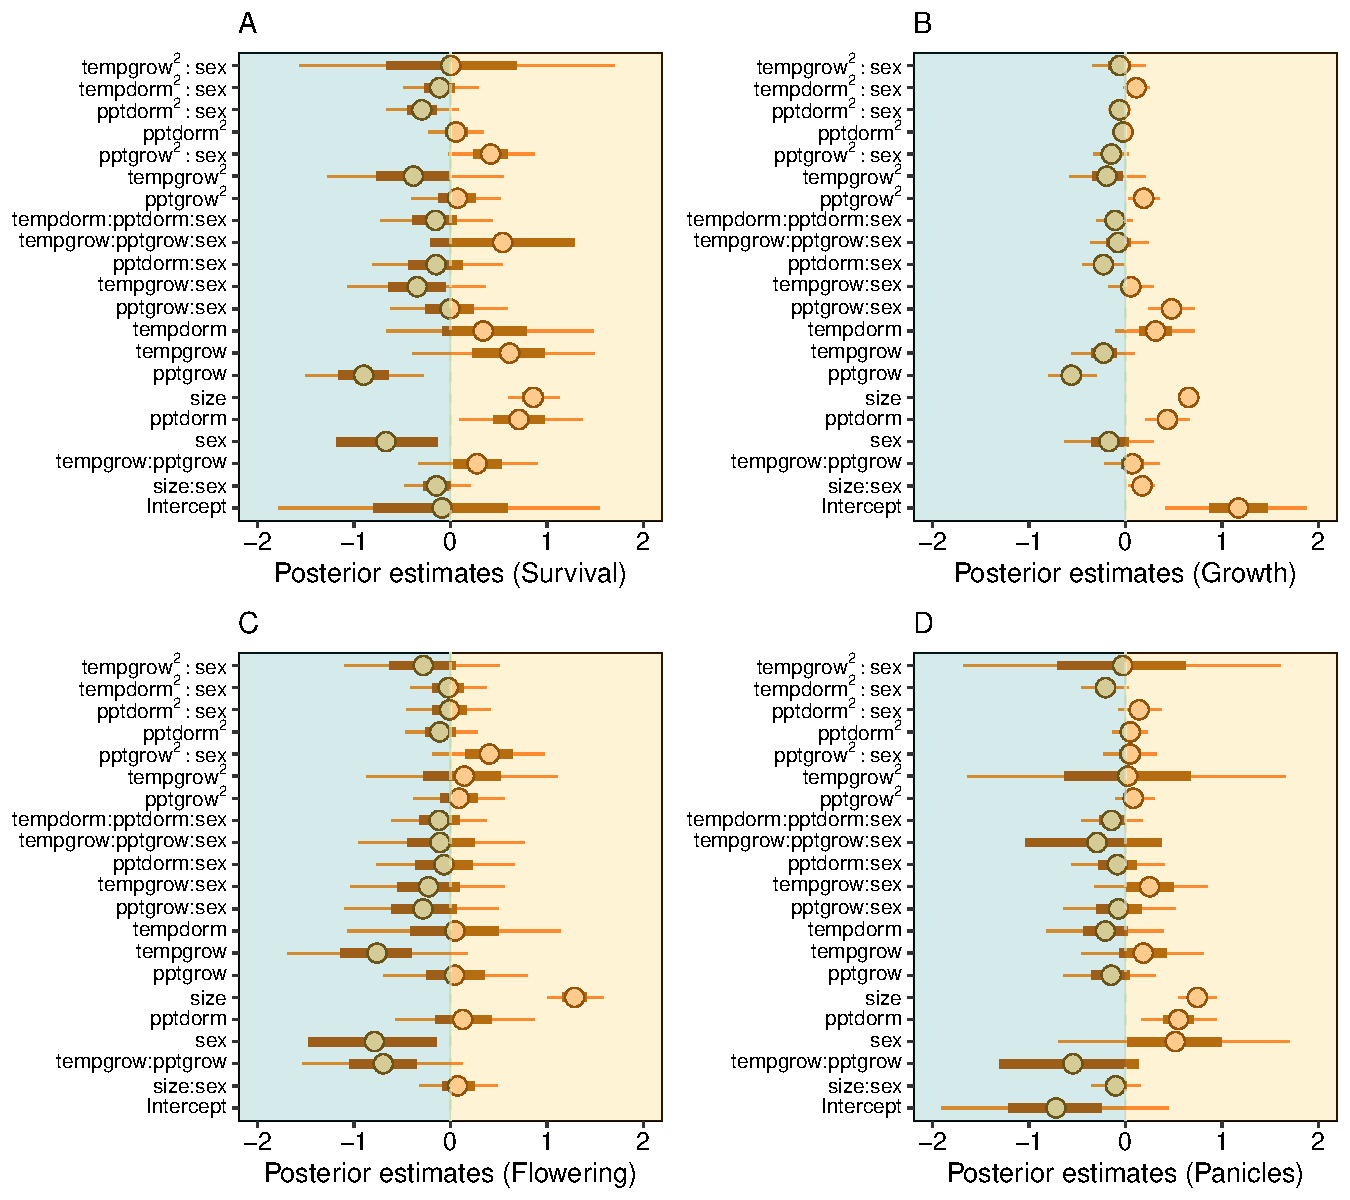
\includegraphics[width=0.99\linewidth]{Figures/Posterior_mean.pdf}
		\caption{Mean parameter values and 95\% credible intervals of the posterior probability distributions. 
		pptgrow is  the precipitation of growing season,
		Tempgrow is the temperature of growing season,
		pptdorm is the temperature of dormant season,
		Tempdorm is the temperature of dormant season.}
		\label{Sup:Posterior}
\end{figure}

\begin{figure}[H]
  \begin{center}
    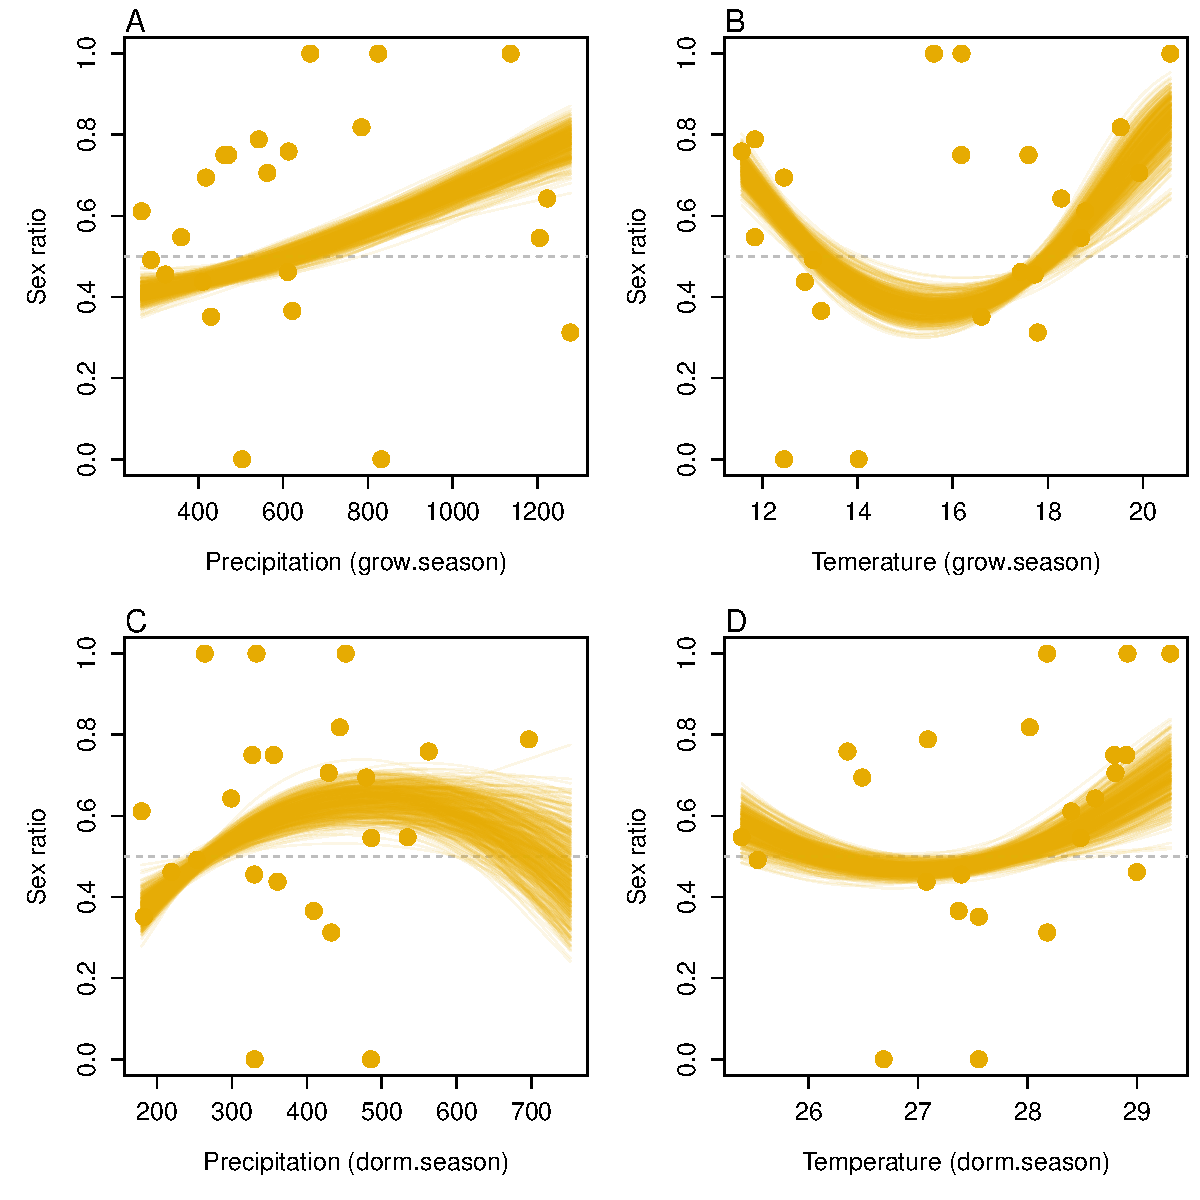
\includegraphics[width=0.80\linewidth]{Figures/gardens_OSR.pdf}
  \caption{\textbf{Significant Operantional Sex Ratio response accross climate gradient}.
  (A, B) Proportion of panicules that were females across precipitation and temperature of the growing season; (C, D) Proportion of of panicules that were females across precipitation and temperature of the dormant season.}
  \label{Sup:gardens_OSR}
  \end{center}
\end{figure}

\begin{figure}[H]
		\centering
		\includegraphics[width=0.75\linewidth]{Figures/Posterior_ORS.pdf}
		\caption{Mean parameter values and 95\% credible intervals of the posterior probability distributions. 
		pptgrow is  the precipitation of growing season,
		Tempgrow is the temperature of growing season,
		pptdorm is the temperature of dormant season,
		Tempdorm is the temperature of dormant season.}
		\label{Sup:PosteriorOSR}
\end{figure}

\begin{figure}[H]
  \begin{center}
    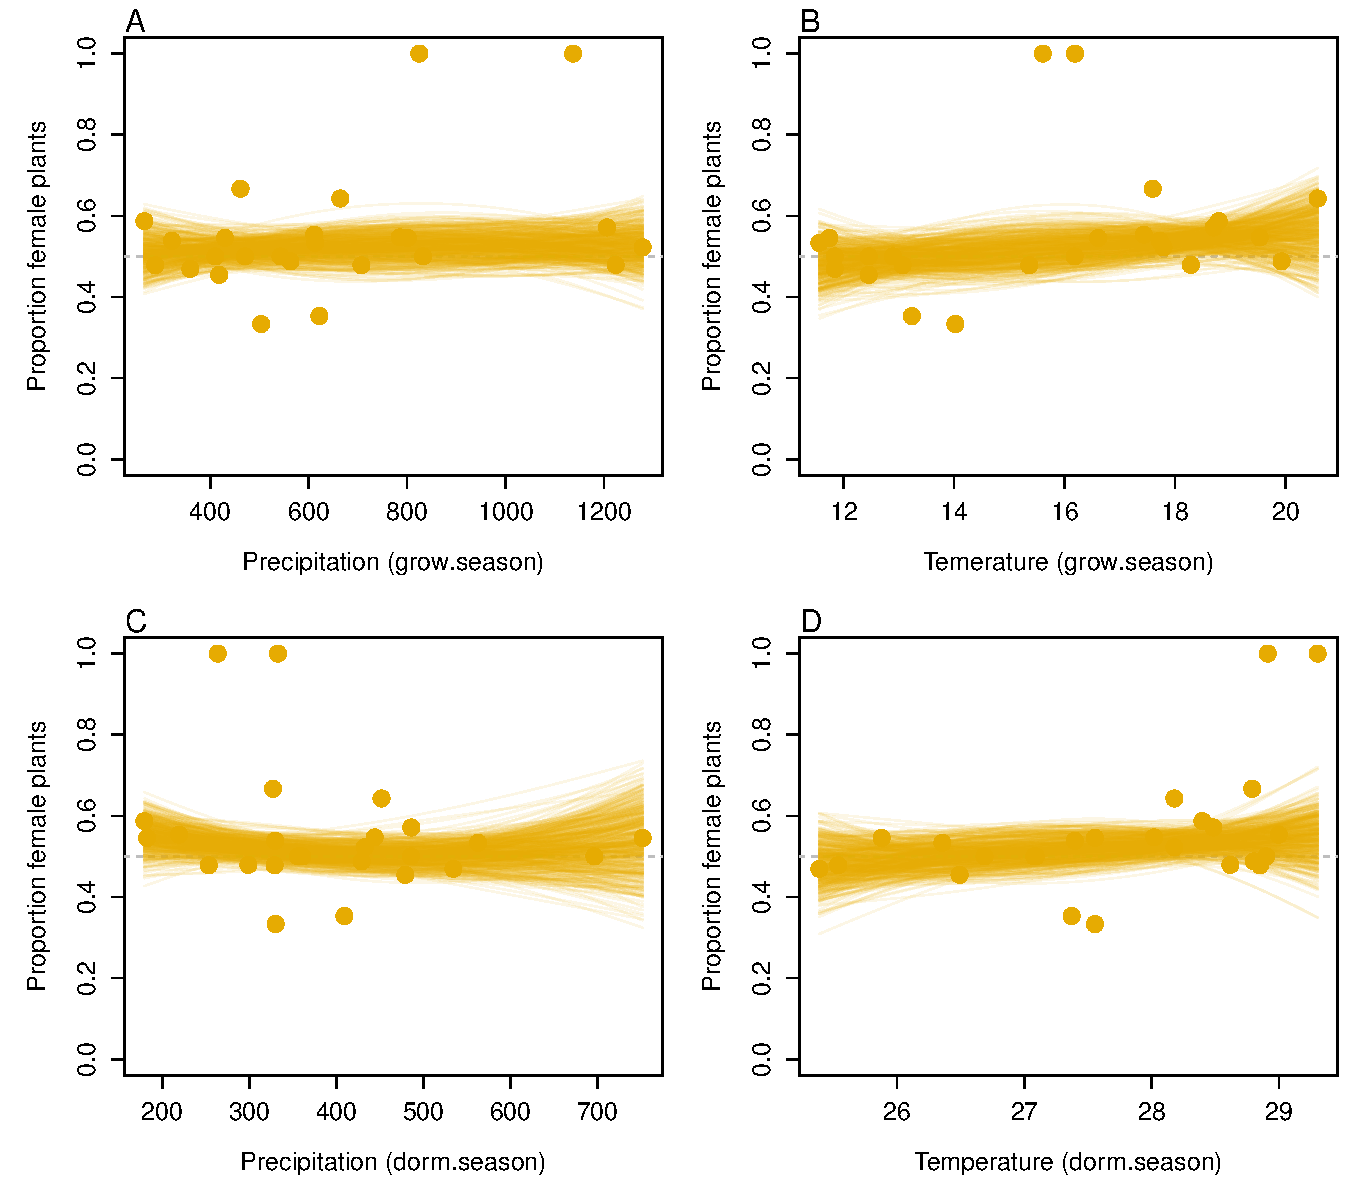
\includegraphics[width=0.95\linewidth]{Figures/gardens_SR.pdf}
  \caption{\textbf{Variation in sex-ratio accross climate gradient}.
  (A, B) Proportion of plants that were females across precipitation and temperature of the growing season; (C, D) Proportion of plants that were females across precipitation and temperature of the dormant season.}
  \label{Sup:gardens_SR}
  \end{center}
\end{figure}

\begin{figure}[H]
		\centering
		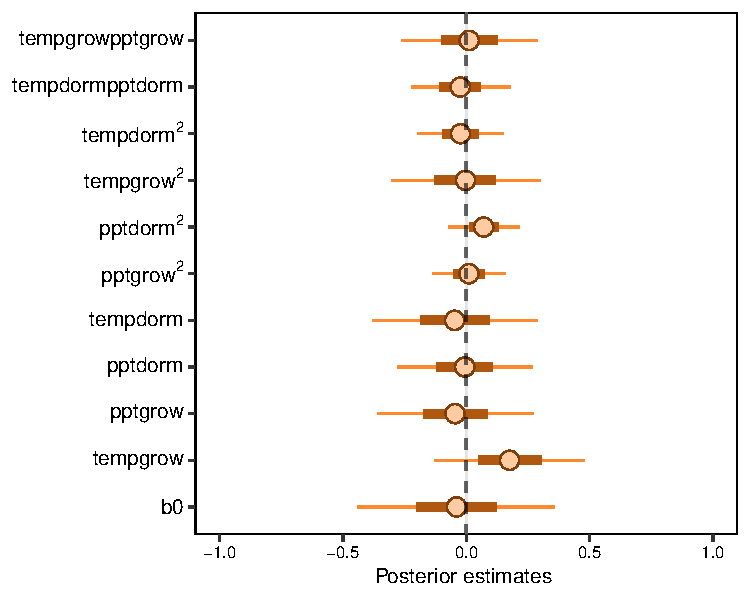
\includegraphics[width=0.75\linewidth]{Figures/Posterior_SR.pdf}
		\caption{Mean parameter values and 95\% credible intervals of the posterior probability distributions. 
		pptgrow is  the precipitation of growing season,
		Tempgrow is the temperature of growing season,
		pptdorm is the temperature of dormant season,
		Tempdorm is the temperature of dormant season.}
		\label{Sup:PosteriorSR}
\end{figure}
	
% \begin{figure}[H]
%   \begin{center}
%     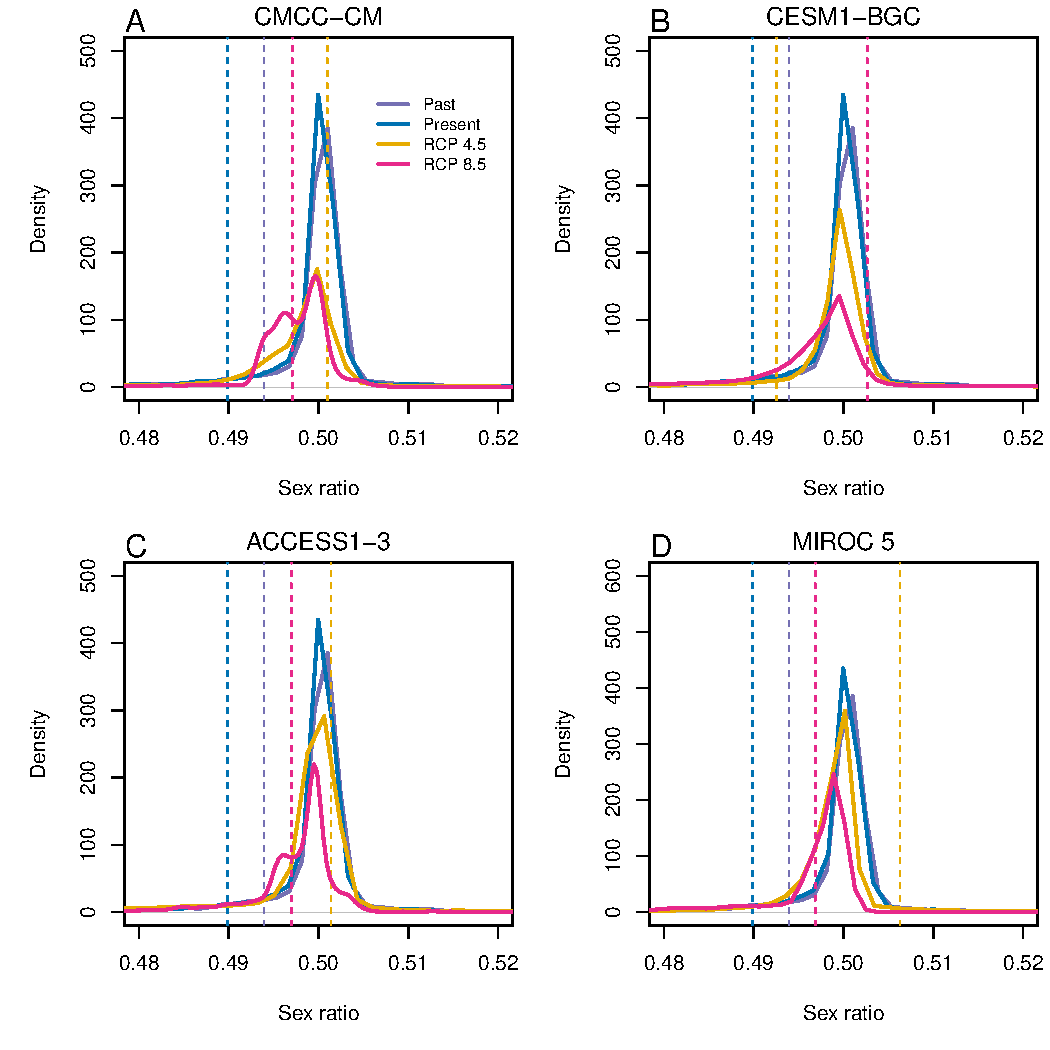
\includegraphics[width=0.99\linewidth]{Figures/POAR_SR.pdf}
%   \caption{Change in Sex ratio (proportion of female) over time (past, present, future).
%   The means for each model are shown as vertical dashed lines.}
%   \label{Sup:srall}
%   \end{center}
% \end{figure}

\begin{figure}[H]
  \begin{center}
    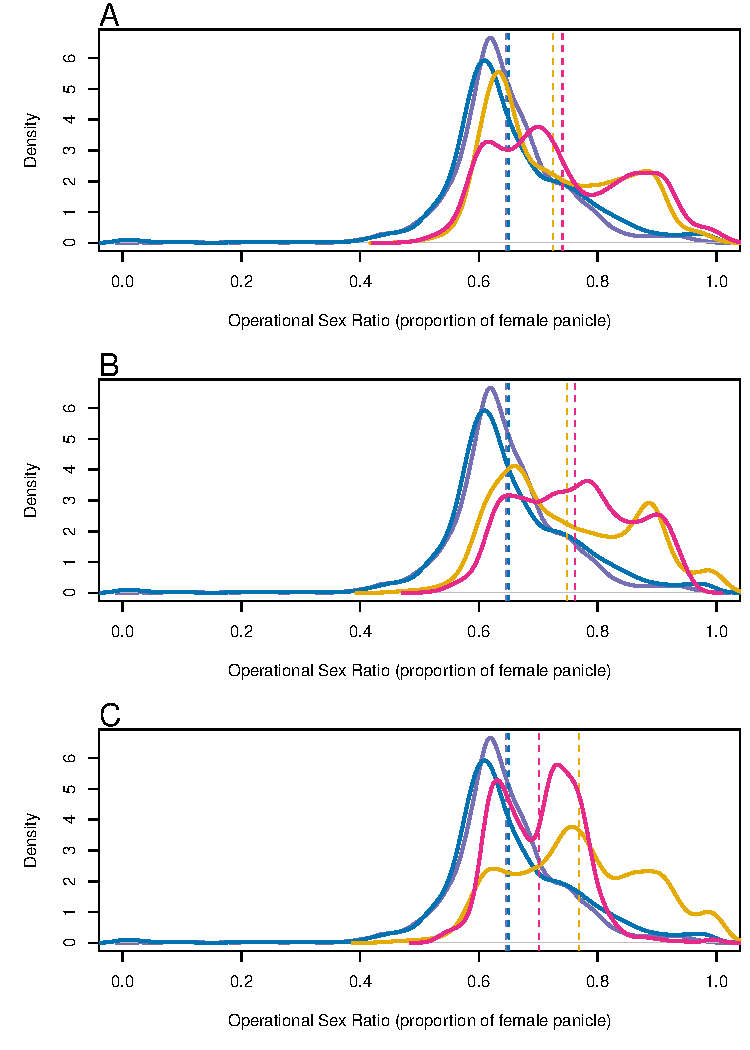
\includegraphics[width=0.80\linewidth]{Figures/POAR_OSR_MIROC_CES_ACC.pdf}
  \caption{Change in Operational Sex Ratio (proportion of female) over time (past, present, future).
  Future projections were based on A) MIROC 5, B) CES, C) ACC.
  The means for each model are shown as vertical dashed lines.}
  \label{Sup:osrall}
  \end{center}
\end{figure}

\begin{figure}[H]
  \begin{center}
    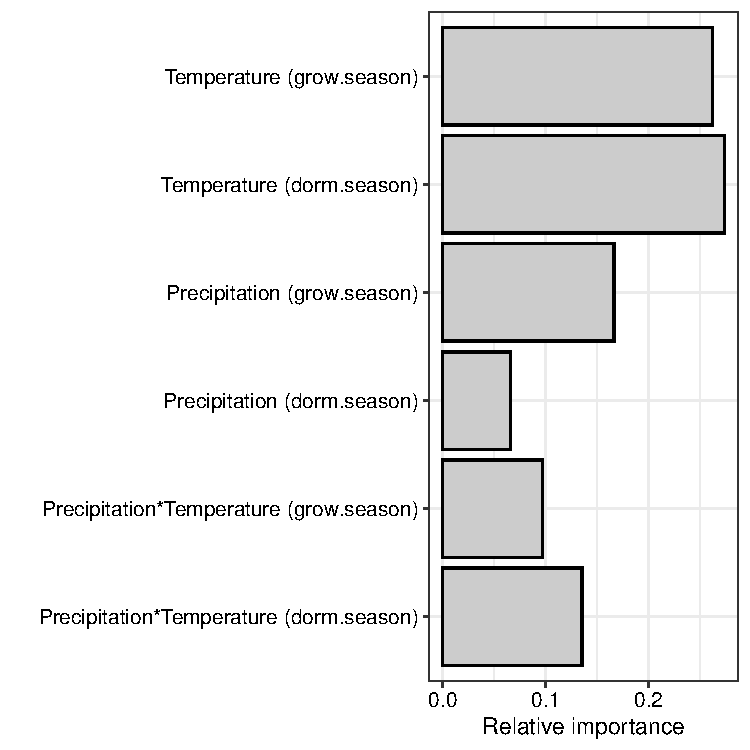
\includegraphics[width=0.65\linewidth]{Figures/Fig_LTRE.pdf}
  \caption{Life Table Response Experiment: The bar represent the relative importance of each predictors.}
  \label{Sup:LTRE}
  \end{center}
\end{figure}

\begin{figure}[H]
  \begin{center}
    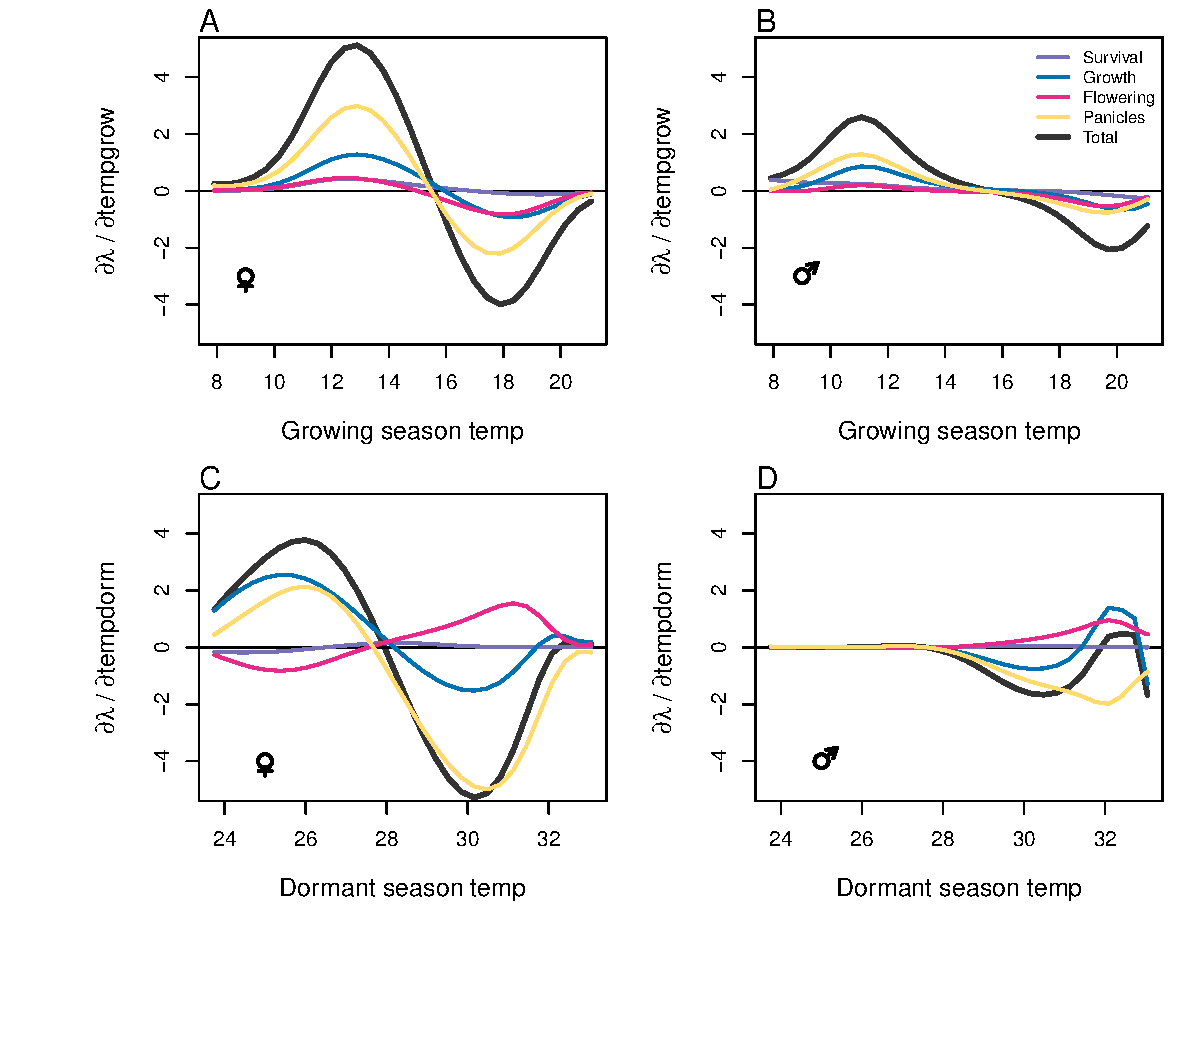
\includegraphics[width=0.95\linewidth]{Figures/LTRE_Temperature.pdf}
  \caption{Life table response experiment decomposition of the sensitivity of $\lambda$ to seasonal climate into additive vital rate contributions of males and females based on posterior mean parameter estimates.
 (A) Temperature of growing season (contribution of female), (B) Temperature of growing season (contribution of male),  (C) Temperature of dormant season (contribution of female) and (D) Temperature of dormant season (contribution of male).}
  \label{Sup:LTRETemp}
  \end{center}
\end{figure}

\begin{figure}[H]
  \begin{center}
    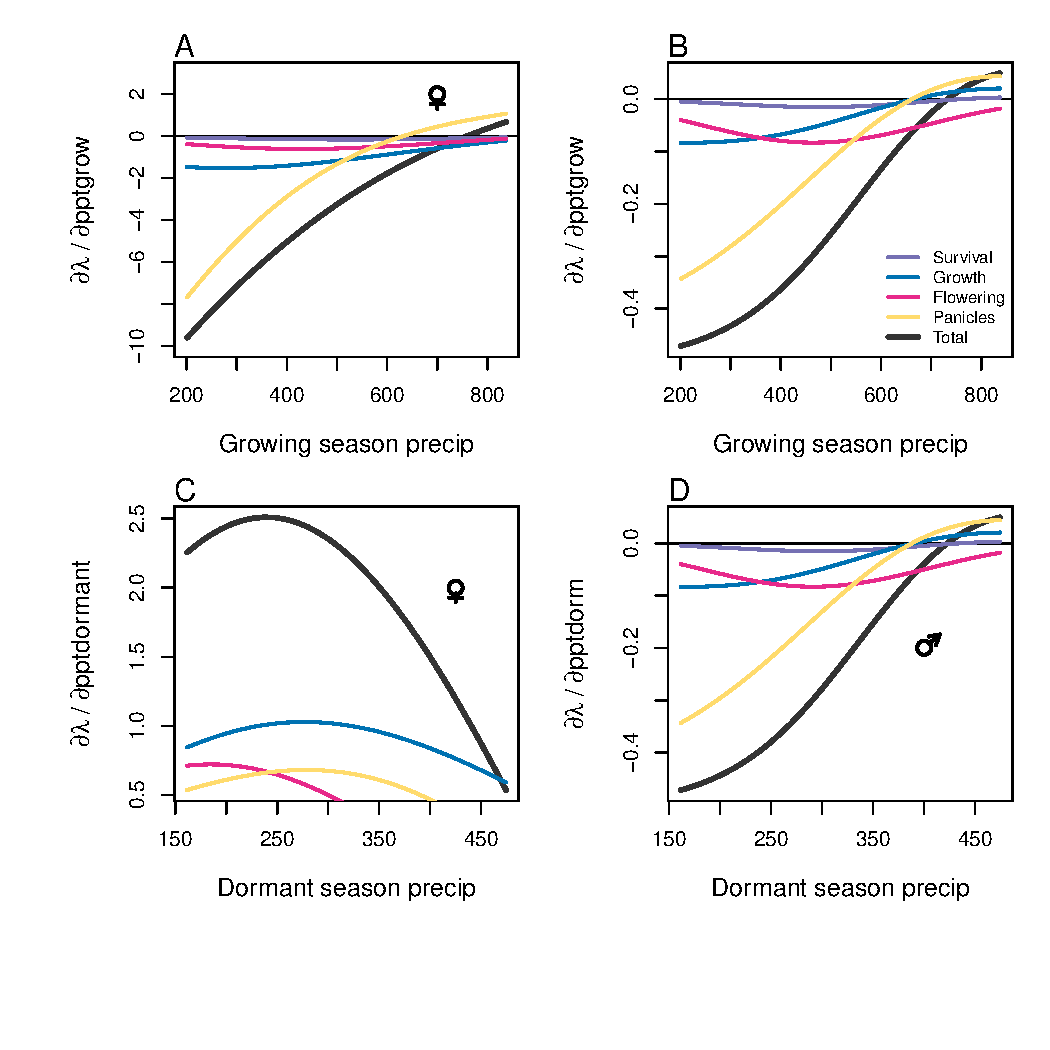
\includegraphics[width=0.95\linewidth]{Figures/LTRE_Precipitation.pdf}
  \caption{Life table response experiment decomposition of the sensitivity of $\lambda$ to seasonal climate into additive vital rate contributions of males and females based on posterior mean parameter estimates.
 (A) Precipitation of growing season (contribution of female), (B) Precipitation of growing season (contribution of male),  (C) Precipitation of dormant season (contribution of female) and (D) Precipitation of dormant season (contribution of male).}
  \label{Sup:LTREppt}
  \end{center}
\end{figure}

\begin{figure}[H]
  \begin{center}
    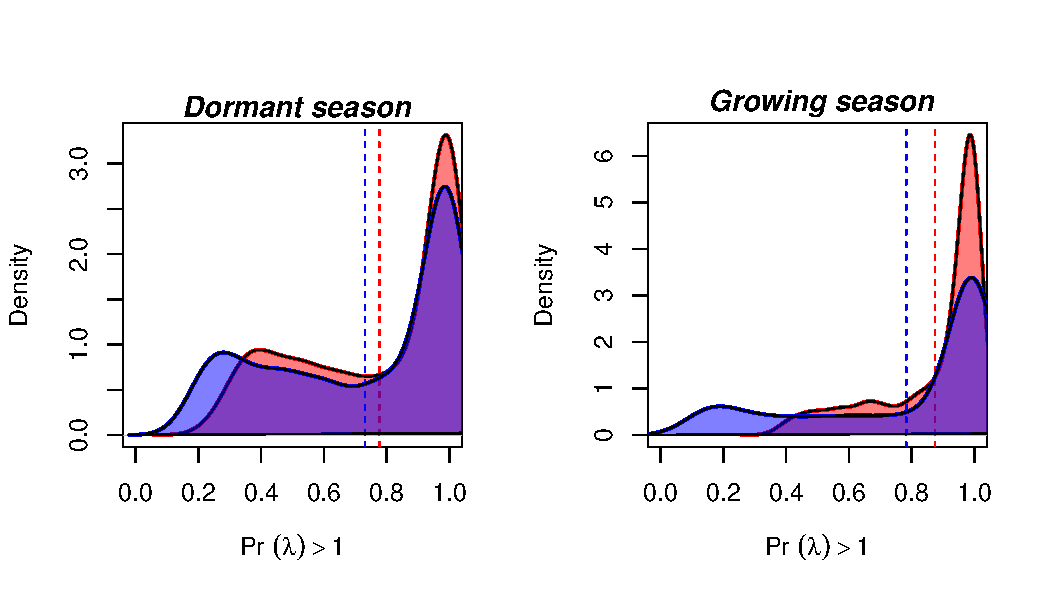
\includegraphics[width=0.99\linewidth]{Figures/Niche_overestimation.pdf}
  \caption{ Assessment of the statistical difference between the two-sex models and the female dominant model for the dormant and growing season. 
  Plots show the density of Pr ($\lambda$) > 1 values for female dominant (pink) and two-sex models (violet) for each season. 
  The means for each model are shown as vertical dashed lines. }
  \label{Sup:Niche_overestimation}
  \end{center}
\end{figure}

% \begin{figure}[H]
%   \begin{center}
%     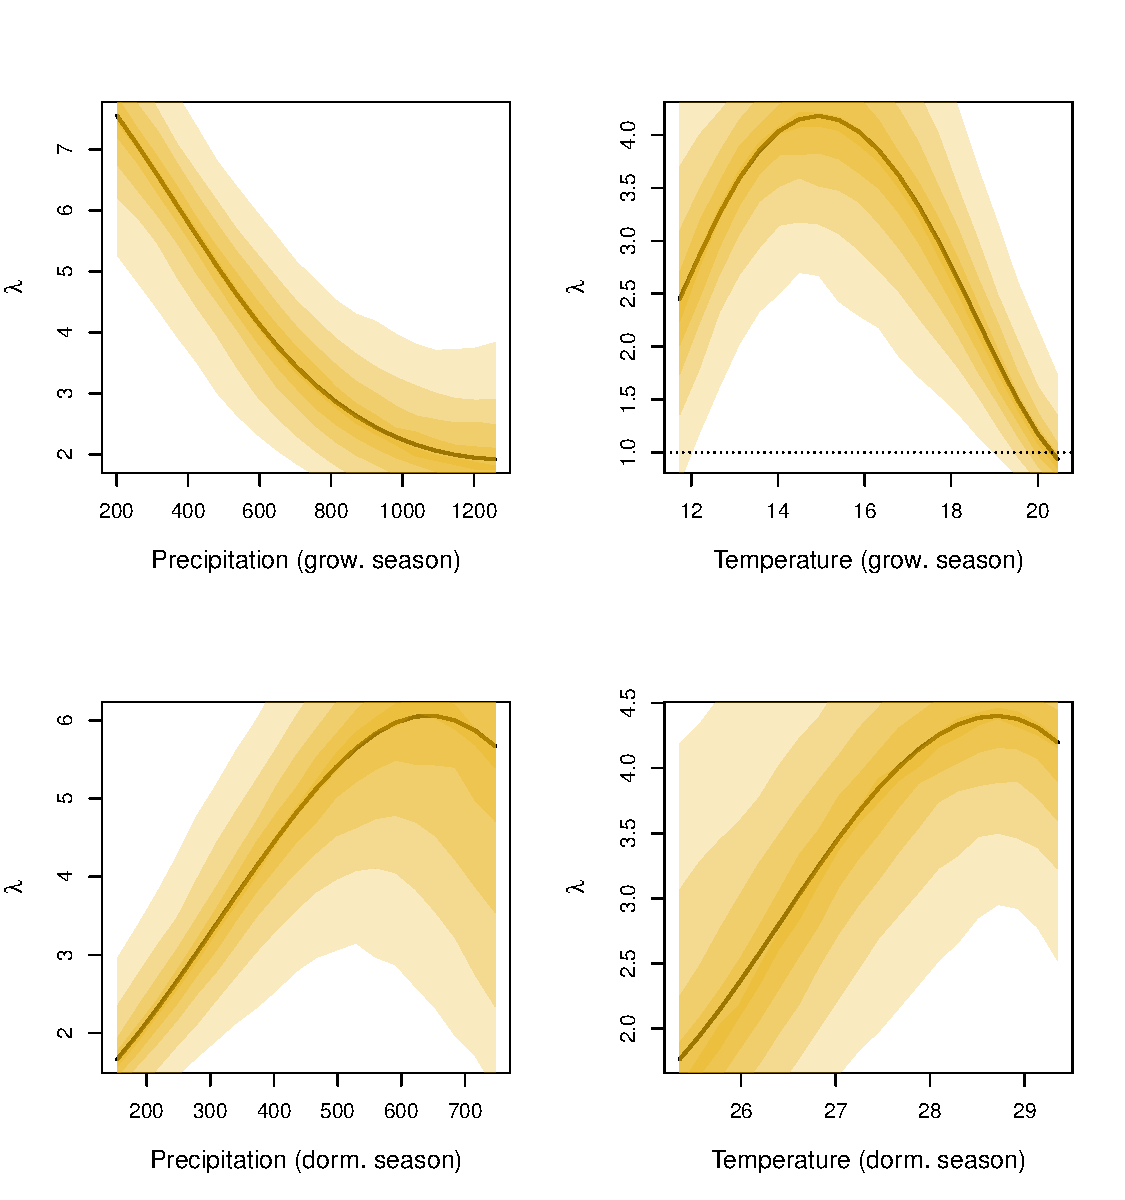
\includegraphics[width=0.95\linewidth]{Figures/lambda_CI.pdf}
%   \caption{Population growth rate ($\lambda$) as a function of seasonal climate (2015-2017), predicted by the two-sex matrix projection model that incorporates sex-specific demographic responses to climate with sex ratio-dependent seed fertilization.
% We show the mean posterior distribution of $\lambda$ in solid lines, and the 5, 25, 50, 75, and 95\% percentiles of parameter uncertainty in shaded gold color.
% The dashed horizontal line indicates the limit of population viability ($\lambda$ = 1)}
%   \label{Sup:lambda2sex}
%   \end{center}
% \end{figure}

\begin{figure}[H]
  \begin{center}
    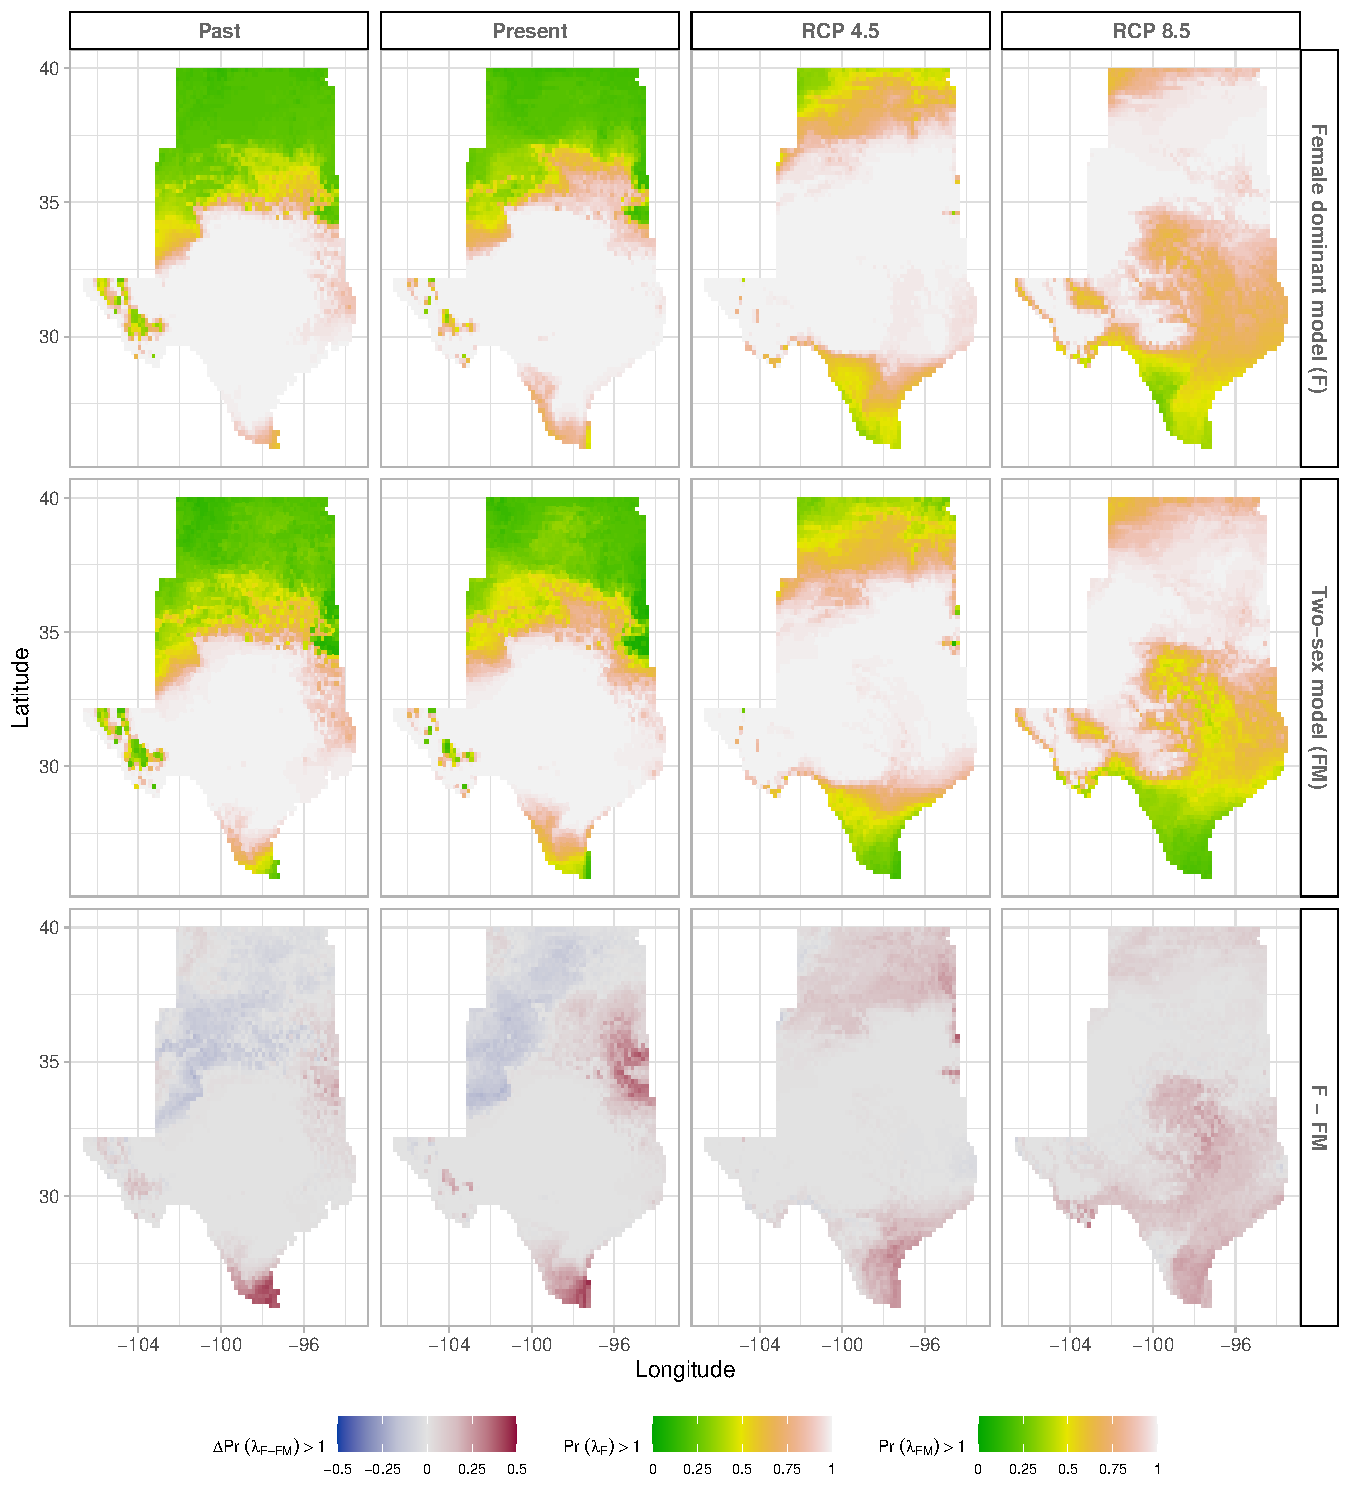
\includegraphics[width=0.95\linewidth]{Figures/Fig_geoPrlambda_ces.pdf}
  \caption{Climate change favors range shift toward the North edge of the current range.
  (A) Past, (B) Current, (C and D) Future predicted range shift based on the predicted probabilities of self- sustaining populations, Pr ($\lambda > 1$), using the two-sex model that incorporates sex- specific demographic responses to climate with sex ratio dependent seed fertilization.
  (E) Past, (F) Current, (G and F) Future  predicted range shift based on the predicted probabilities of self- sustaining populations, Pr ($\lambda > 1$), using the female dominant model.
  Future projections were based on the CESM1-BGC model.
  The black dots on panel B and F indicate all known presence points collected from GBIF from 1990 to 2019, which corresponds to the current condition in our prediction. 
  The occurrences of GBIFs are distributed in with higher population fitness habitat Pr ($\lambda$ > 1) , confirming that our study approach can reasonably predict range shifts. }
  \label{Sup:geoprojces}
  \end{center}
\end{figure}

\begin{figure}[H]
  \begin{center}
    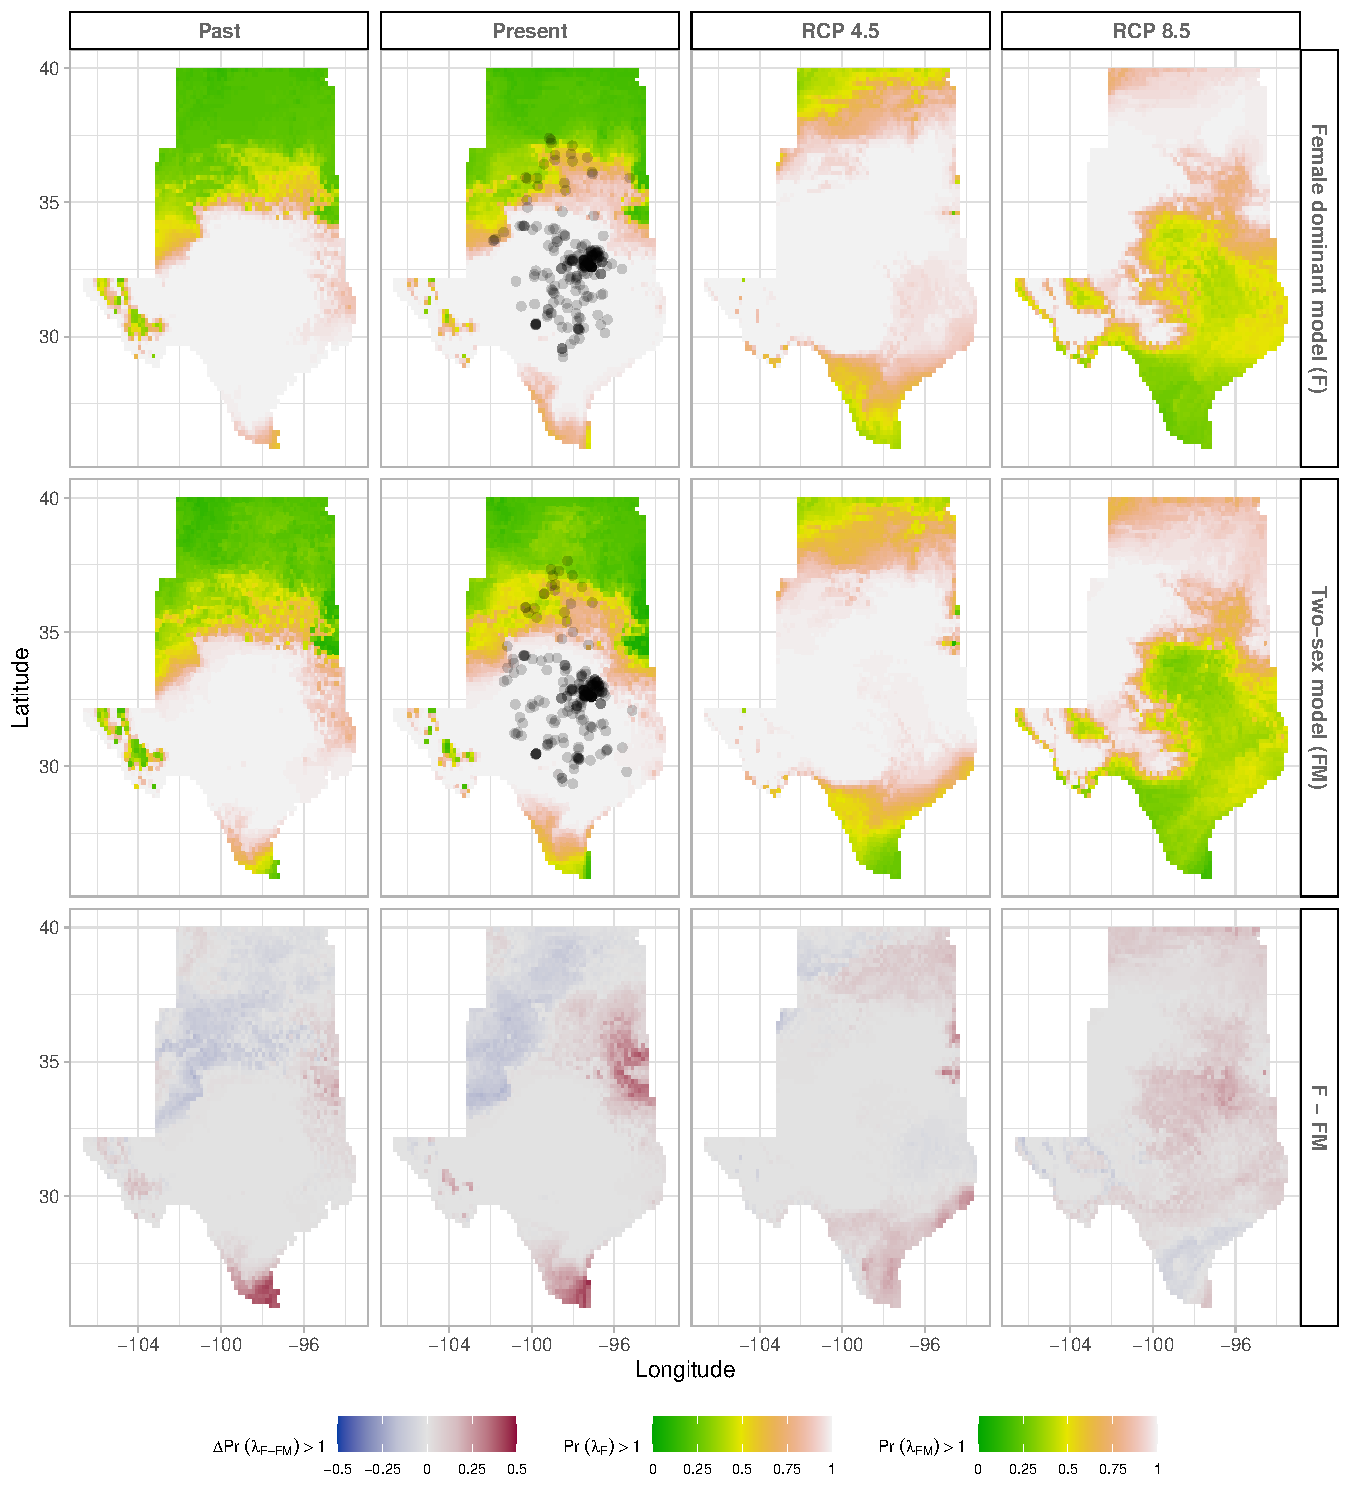
\includegraphics[width=0.95\linewidth]{Figures/Fig_geoPrlambdaacc.pdf}
  \caption{Climate change favors range shift toward the North edge of the current range.
  (A) Past, (B) Current, (C and D) Future predicted range shift based on the predicted probabilities of self- sustaining populations, Pr ($\lambda > 1$), using the two-sex model that incorporates sex- specific demographic responses to climate with sex ratio dependent seed fertilization.
  (E) Past, (F) Current, (G and F) Future  predicted range shift based on the predicted probabilities of self- sustaining populations, Pr ($\lambda > 1$), using the female dominant model.
  Future projections were based on the  ACCESS model.
  The black dots on panel B and F indicate all known presence points collected from GBIF from 1990 to 2019, which corresponds to the current condition in our prediction. 
  The occurrences of GBIFs are distributed in with higher population fitness habitat Pr ($\lambda$ > 1) , confirming that our study approach can reasonably predict range shifts.}
  \label{Sup:geoprojcmc}
  \end{center}
\end{figure}

\begin{figure}[H]
  \begin{center}
    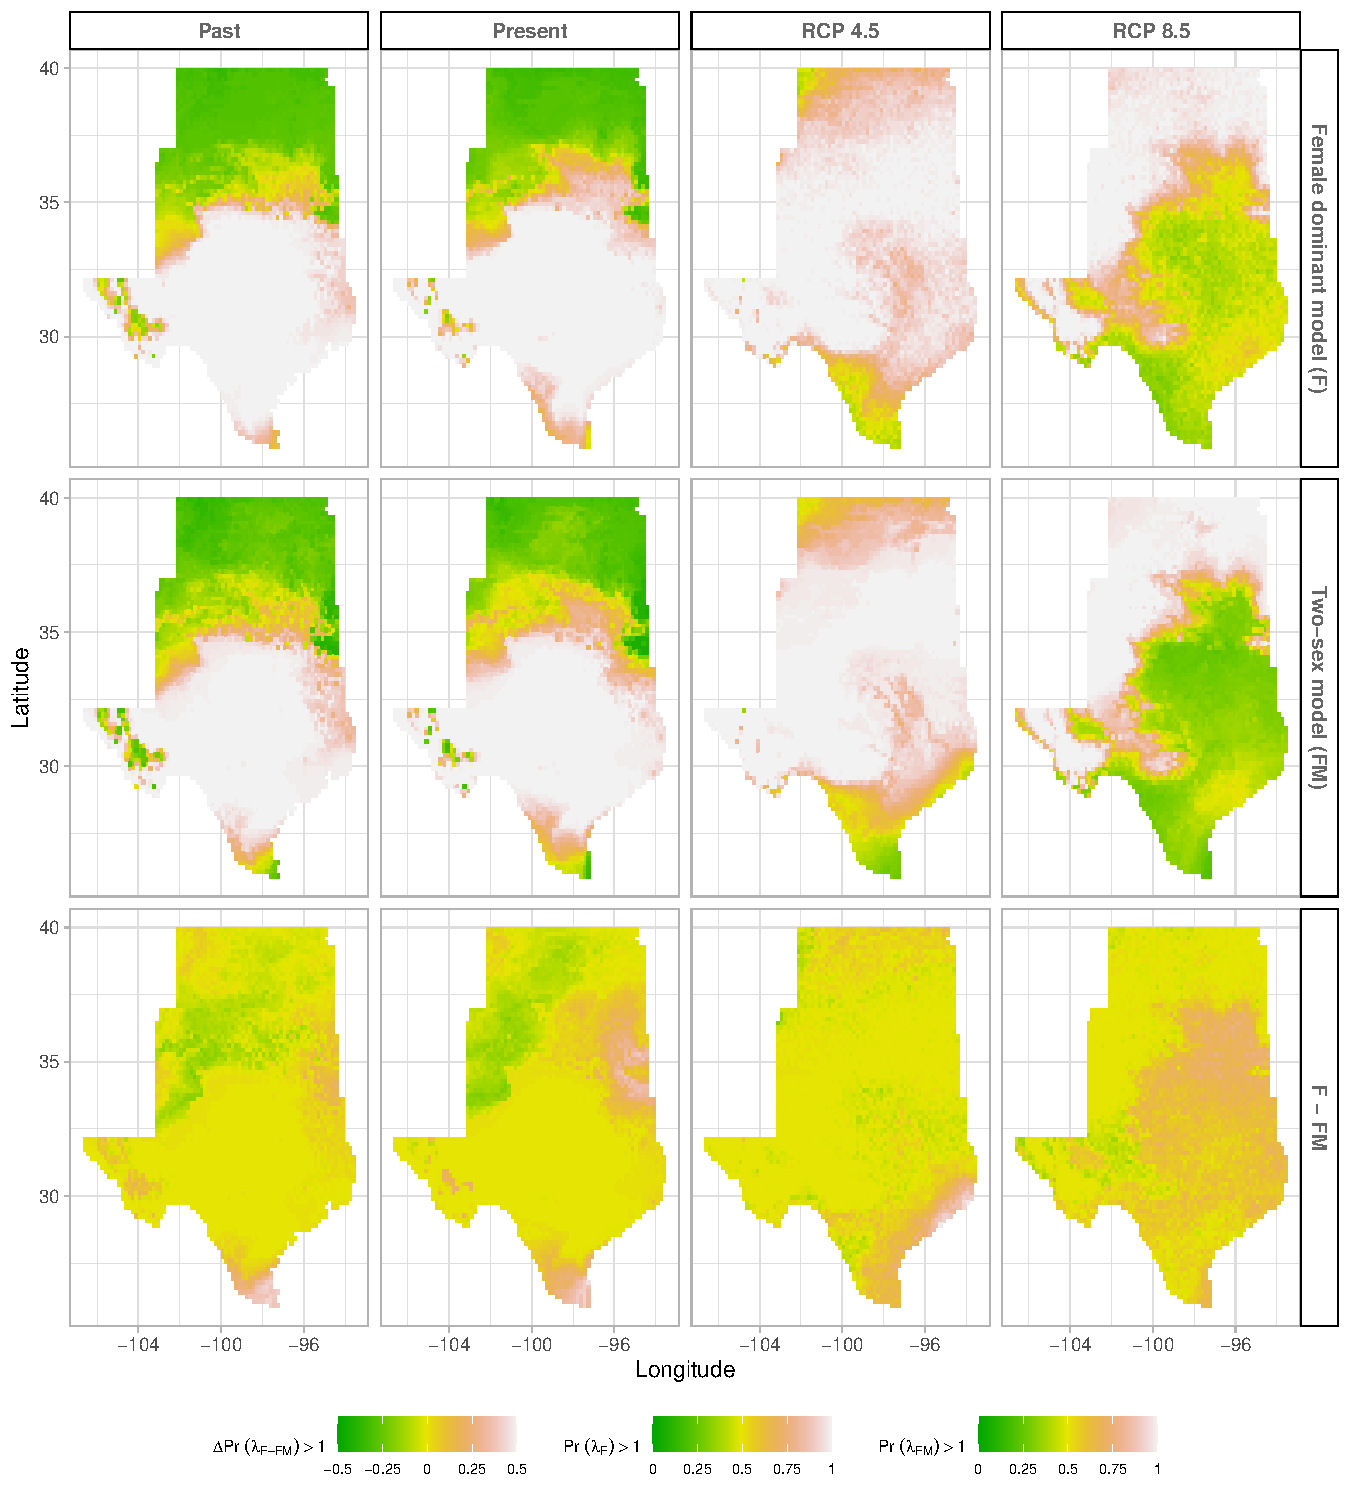
\includegraphics[width=0.95\linewidth]{Figures/Fig_geoPrlambda_miroc.pdf}
  \caption{Climate change favors range shift toward the North edge of the current range.
  (A) Past, (B) Current, (C and D) Future predicted range shift based on the predicted probabilities of self- sustaining populations, Pr ($\lambda > 1$), using the two-sex model that incorporates sex- specific demographic responses to climate with sex ratio dependent seed fertilization.
  (E) Past, (F) Current, (G and F) Future  predicted range shift based on the predicted probabilities of self- sustaining populations, Pr ($\lambda > 1$), using the female dominant model.
  Future projections were based on the MIROC5 model.
  The black dots on panel B and F indicate all known presence points collected from GBIF from 1990 to 2019, which corresponds to the current condition in our prediction. 
  The occurrences of GBIFs are distributed in with higher population fitness habitat Pr ($\lambda$ > 1) , confirming that our study approach can reasonably predict range shifts.}
  \label{Sup:geoprojmiroc}
  \end{center}
\end{figure}


% \begin{figure}[H]
%   \begin{center}
%     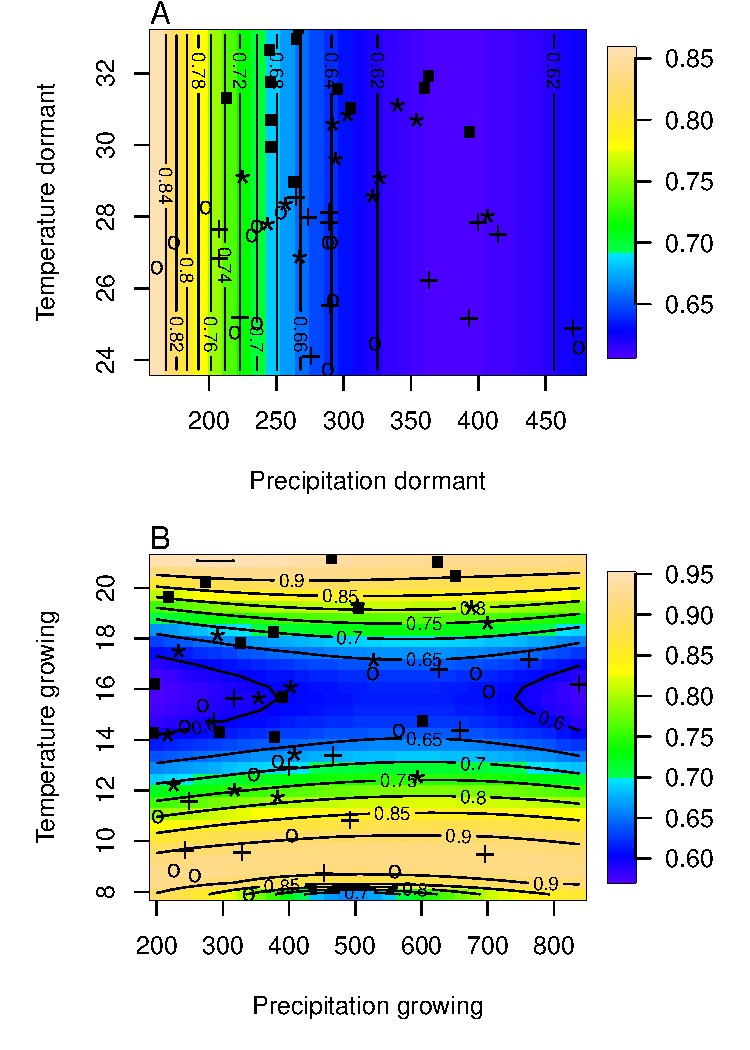
\includegraphics[width=0.75\linewidth]{Figures/OSR.pdf}
%   \caption{A two‐dimensional representation of the Operational Sex Ratio (OSR) over time (past, present and future climate conditions). 
%   OSR represents the proportion of females. 
%   Contours show predicted values of OSR conditional on precipitation and temperature of the dormant and growing season.
%   Operational Sex Ratio during the dormant season for the two sex model (A), Operational Sex Ratio during the growing season for the two sex model (B).
%   "\begin{normalsize}\textbf{o}\end{normalsize}": Past, "\begin{normalsize}\textbf{+}\end{normalsize}": Current,"\begin{large}\textbf{*}\end{large}": RCP 4.5,"\begin{tiny}$\blacksquare$\end{tiny}": RCP 8.5.}
%   \label{Sup:OSR}
%   \end{center}
% \end{figure}

% \begin{figure}[H]
%   \begin{center}
%     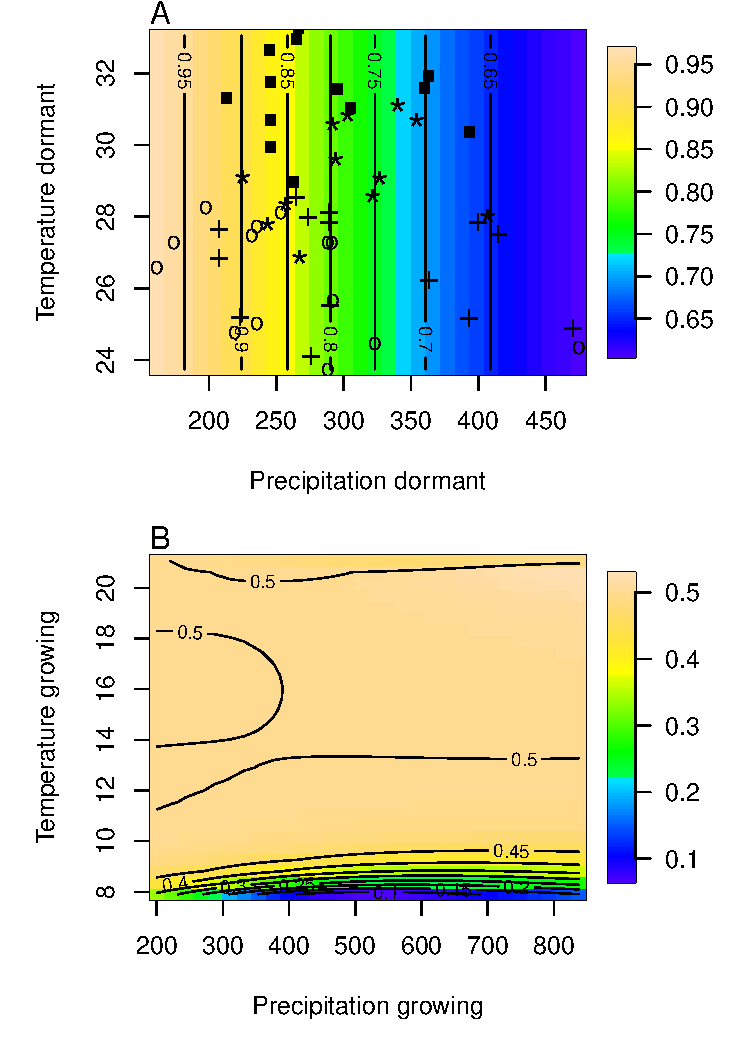
\includegraphics[width=0.85\linewidth]{Figures/SR.pdf}
%   \caption{A two‐dimensional representation of the  Sex Ratio (SR) over time (past, present and future climate conditions). 
%   Contours show predicted values of SR conditional on precipitation and temperature of the dormant and growing season.
%   Sex Ratio during the dormant season for the two sex model (A),Sex Ratio during the growing season for the two sex model (B).}
%   \label{Sup:SR}
%   \end{center}
% \end{figure}

\section {Supporting Methods}

\subsection*{Sex ratio experiment}
\label{sec:experiment}
To estimate the probability of seed viability,  the germination rate and the effect of sex-ratio variation on female reproductive success, we conducted a sex-ratio experiment at one site near the center of the range to estimate the effect of sex-ratio variation on female reproductive success.
The details of the experiment are provided in \cite{compagnoni2017can} and \cite{miller2022two}.
Here we provide a summary of the experiment.
We established 124 experimental populations in plots measuring 0.4 x 0.4m and separated by at least 15m from each other.
We varied population density (1-48 plants/plot) and sex ratio (0\%-100\% female) across the experimental populations, and we replicated 34 combinations of density and sex ratio.
We collected panicles from a subset of females in each plot and recorded the number of seeds in each panicle.
We assessed reproductive success (seeds fertilized) using greenhouse-based germination and trazolium-based seed viability assays.
Seed viability was modeled with a binomial distribution where the probability of viability ($v$) was given by:
\begin{align}\label{eq:viab}
v = v_{0} * (1 - OSR^{\alpha})
\end{align}
\noindent where $OSR$ is the proportion of panicles that were female in the experimental populations.
% The properties of the above function is supported by our previous work \citep{compagnoni2017can}.
% Here, seed viability is maximized at $v_{0}$ as $OSR$ approaches zero (strongly male-biased) and goes to zero as $OSR$ approaches $1$ (strongly female-biased).
$\alpha$ is the parameter that control for how viability declines with increasing female bias.
Further, germination rate was modeled using a binomial distribution to model the germination data from greenhouse trials.
Given that germination was conditional on seed viability,the probability of success was given by the product $v*g$, where $v$ is a function of $OSR$ (Eq. \ref{eq:viab}) and $g$ is assumed to be constant.


\end{document}
